\chapter{Background}

The introductory material we provide in this section sets up the scene for the work that will be later explained. It follows a path that goes from the early days of program reasoning all the way to modern techniques that allow to deal with concurrency. On top of this, we look at database theory from a transactional perspective, analyzing concurrency control paradigms and consistency models.

\section{History of Concurrent Reasoning}

Before entering the world of modern program logics for concurrency, we study the building blocks that serve as its foundation. First and foremost, the work done by Tony Hoare provides us with the starting point for reasoning about sequential programs using an axiomatic approach. The latter is expanded in order to cope with concurrency, and later enhanced through a methodology allowing the abstraction of effects that concurrent threads may have on the program state.

\tocless\subsection{Hoare Logic}

As a starting point in proving correctness, or generally properties of computer programs, Hoare \cite{hoare} explains how to use deductive reasoning in applying inference rules to a set of predefined language axioms. He specifies the use of what was later on referred to as a ``Hoare triple" of the shape $\triple{P}{C}{Q}$ where $P$ and $Q$ are first-order assertions while $C$ is the program executed. $P$ is called the precondition of $C$ while $Q$ is its postcondition. The triple thus describes that whenever the assertion $P$ holds before $C$ runs and at some point terminates, then $Q$ will hold on its completion. The kind of logic adopted, allows to reason about relatively simple programs involving integers and local variables living in the \textit{stack} of a function. Classic proofs performed using Hoare logic take the form of a proof tree with axioms as leaves and rules as intermediate steps. Such notation has the downside that complete proofs tend to explode in size. For this reason, proof sketches are utilized. They represent the holding assertions before and after every command that appears in the analyzed code. We can see an example of such in Figure \ref{fig:abshoare}.
\begin{center}
	\begin{gather*}
		\begin{array}{l}
		\specline{\top} \\
		\pfunctions{abs}{\pvar{x}} \\
			\quad \passign{\pvar{r}}{\pvar{x}}; \\
			\quad \specline{\pvar{x} = \pvar{r}} \\
			\quad \pifelses{\pvar{x} < 0} \\
				\quad \quad \specline{\pvar{x} < 0 \land \pvar{x} = \pvar{r}} \\
				\quad \quad \passign{\pvar{r}}{-\pvar{x}}; \\
				\quad \quad \specline{\pvar{x} < 0 \land \pvar{r} = - \pvar{x}} \\
				\quad \quad \specline{(\pvar{x} < 0 \land \pvar{r} = -\pvar{x}) \lor (\pvar{x} \geq 0 \land \pvar{r} = \pvar{x})} \\
			\quad \pifelsem \\
				\quad \quad \specline{\pvar{x} \geq 0 \land \pvar{x} = \pvar{r}} \\
				\quad \quad \pskip; \\
				\quad \quad \specline{\pvar{x} \geq 0 \land \pvar{x} = \pvar{r}} \\
				\quad \quad \specline{(\pvar{x} < 0 \land \pvar{r} = -\pvar{x}) \lor (\pvar{x} \geq 0 \land \pvar{r} = \pvar{x})} \\
			\quad \pifelsee \\
			\quad \specline{(\pvar{x} < 0 \land \pvar{r} = -\pvar{x}) \lor (\pvar{x} \geq 0 \land \pvar{r} = \pvar{x})} \\
			\quad \preturn{\pvar{r}}; \\
		\pfunctione \\
		\specline{(\pvar{x} < 0 \land \pvar{ret} = -\pvar{x}) \lor (\pvar{x} \geq 0 \land \pvar{ret} = \pvar{x})} \\
		\end{array}
	\end{gather*}
	\captionof{figure}{A proof sketch of the absolute value function using Hoare logic.}
	\label{fig:abshoare} 
\end{center}

The $\mathtt{abs}(\pvar{x})$ function simply returns the absolute value of the input argument $\pvar{x}$. We notice that the procedure's precondition is $\top$ ($true$), which means that there is no particular assertion which needs to hold in order for the code to perform its task. On the other hand, the postcondition states that the return value, which is referred to using a special variable named $\pvar{ret}$, will effectively be the absolute value of $\pvar{x}$. Note how the postcondition of every command in a sequence becomes the precondition of the following one, respecting the rule specified in \cite{hoare}.

\tocless\subsection{Owicki-Gries}

In a concurrent setting, the first approach that allowed reasoning of programs was presented in \cite{owicki} and is referred to as the ``Owicki-Gries" method from the name of its authors. Its main contribution is the parallel composition rule.

\[
	\infer[\textsc{Owicki-Gries}]
	{
		\vdash \triple{P_1 \land P_2}{C_1\ ||\ C_2}{Q_1 \land Q_2}
	}
	{
		\vdash \triple{P_1}{C_1}{Q_1} &
		\vdash \triple{P_2}{C_2}{Q_2} &
		\textsf{interference-free}
	}
\]

The rule states that we perform a regular sequential proof for each of the threads that are composed together and the resulting postcondition will be the conjunction of all the components' ones. This holds as long as the proofs of the individual thread runs are not interfering with each other. In other words, every intermediate assertion between atomic commands in the sequential proof of $C_1$ must be kept valid by the actions of $C_2$ and vice versa \cite{viktor}.
\begin{center}
\[\footnotesize
\begin{array}{c}
\infer[\textsc{Cons}]
{
	\triple
	{\pvar{x} = 0}
	{\passign{\pvar{x}}{\pvar{x} + 1}\ ||\ \passign{\pvar{x}}{\pvar{x} + 2}}
	{\pvar{x} = 3}
}
{
	\infer[\textsc{Owicki-Gries}]
	{
		\triple
		{\pvar{x} = 0 \land \pvar{x} = 0}
		{\passign{\pvar{x}}{\pvar{x} + 1}\ ||\ \passign{\pvar{x}}{\pvar{x} + 2}}
		{(\pvar{x} = 1 \lor \pvar{x} = 3) \land (\pvar{x} = 2 \lor \pvar{x} = 3)}
	}
	{
		(\dag)
		\ \ \ \ \ \ \ \ \ \ \ \ \ \ \ \	
		(\spadesuit)
	}
}
\\[1.5em]
(\dag) =
\infer[\textsc{Cons}]
		{
			\triple
			{\pvar{x} = 0}
			{\passign{\pvar{x}}{\pvar{x} + 1}}
			{\pvar{x} = 1 \lor \pvar{x} = 3}
		}
		{
			\infer[\textsc{Assign}]
			{
				\triple
				{\pvar{x} = 0 \lor \pvar{x} = 2}
				{\passign{\pvar{x}}{\pvar{x} + 1}}
				{\pvar{x} = 1 \lor \pvar{x} = 3}
			}
			{\ldots}		
		}
\\[1.5em]
(\spadesuit) = 
\infer[\textsc{Cons}]
		{
			\triple
			{\pvar{x} = 0}
			{\passign{\pvar{x}}{\pvar{x} + 2}}
			{\pvar{x} = 2 \lor \pvar{x} = 3}
		}
		{
			\infer[\textsc{Assign}]
			{
				\triple
				{\pvar{x} = 0 \lor \pvar{x} = 1}
				{\passign{\pvar{x}}{\pvar{x} + 2}}
				{\pvar{x} = 2 \lor \pvar{x} = 3}
			}
			{\ldots}		
		}
\\[1.5em]
\infer[\textsc{Cons}]
	{
		\triple
		{P}
		{C}
		{Q}
	}
	{
		P \Rightarrow P' &
		\triple
		{P'}
		{C}
		{Q'} &
		Q' \Rightarrow Q
	}
\end{array}
\]
\captionof{figure}{Partial proof tree of a parallel program incrementing variable $\pvar{x}$ which also uses the \textsc{Cons} rule (provided).}
\end{center}

The method's main burden is the \textsf{interference-free} constraint which makes non-trivial commands very complicated to prove. As a consequence, most specifications that satisfy the requirement will be too weak to prove any interesting properties about the concurrent code. This is the reason why such a method is only able to give stronger specifications using auxiliary or ghost variables whose task is to keep track of past program states. In addition, the actual code needs to be augmented with statements that refer to the ghost variables themselves. Any modular use of proofs that involve auxiliary variables would require new specifications, since the number of variables needed to express strong specifications would increase based on the way the module is used (e.g. the number of threads running). This becomes clear by looking at an example of two threads incrementing the same counter concurrently. We first define the counter's methods and then show a summarized proof of clients' usage through ghost variables \cite{modularsteps}.
\begin{gather*}
\begin{array}{@{}l@{\qquad}l@{\qquad}l@{}}
\begin{array}{@{}l@{}}
\pfunctions{makeCounter}{} \\
\quad \palloc{\pvar{c}}{1}; \\
\quad \pmutate{\pvar{c}}{0}; \\
\quad \preturn{\pvar{c}}; \\
\pfunctione
\end{array}
&
\begin{array}{@{}l@{}}
\pfunctions{increment}{\pvar{c}} \\
\quad \texttt{do } \{ \\
	\quad \quad \pderef{\pvar{n}}{\pvar{c}}; \\
	\quad \quad \pfuncall{\pvar{b}}{CAS}{\pvar{c}, \pvar{n}, \pvar{n} + 1}; \\
\quad \} \texttt{ while }(\pvar{b} = 0); \\
\quad \preturn{\pvar{n}}; \\
\pfunctione
\end{array}
\end{array} \\ \\
\pfuncall{\pvar{c}}{makeCounter}{};
\color{ForestGreen}\passign{\pvar{inc}_1}{0};
\passign{\pvar{inc}_2}{0}; \\
\color{blue} \{ \cell{\pvar{c}}{0} \land \pvar{inc}_1 = 0 \land \pvar{inc}_2 = 0 \} \\
\begin{array}{c || c}
\begin{array}{l}
\color{blue} \{ \cell{\pvar{c}}{\pvar{inc}_1 + \pvar{inc}_2} \land \pvar{inc}_1 = 0 \} \\
\texttt{do } \{ \\
	\quad \pderef{\pvar{n}}{\pvar{c}}; \\
	\quad \patomic{\pfuncall{\pvar{b}}{CAS}{\pvar{c}, \pvar{n}, \pvar{n} + 1}; \\
		\quad \quad \textcolor{ForestGreen}{\pifelses{\pvar{b}} \pvar{inc}_1\texttt{++}\pifelsee}} \\
\} \texttt{ while }(\pvar{b} = 0); \\
\color{blue} \{ \cell{\pvar{c}}{\pvar{inc}_1 + \pvar{inc}_2} \land \pvar{inc}_1 = 1 \} \\
\end{array}
&
\begin{array}{l}
\color{blue} \{ \cell{\pvar{c}}{\pvar{inc}_1 + \pvar{inc}_2} \land \pvar{inc}_2 = 0 \} \\
\texttt{do } \{ \\
	\quad \pderef{\pvar{n}'}{\pvar{c}}; \\
	\quad \patomic{\pfuncall{\pvar{b}'}{CAS}{\pvar{c}, \pvar{n}', \pvar{n}' + 1}; \\
		\quad \quad \textcolor{ForestGreen}{\pifelses{\pvar{b}'} \pvar{inc}_2\texttt{++}\pifelsee}} \\
\} \texttt{ while }(\pvar{b}' = 0); \\
\color{blue} \{ \cell{\pvar{c}}{\pvar{inc}_1 + \pvar{inc}_2} \land \pvar{inc}_2 = 1 \} \\
\end{array}
\end{array} \\
\color{blue} \{ \cell{\pvar{c}}{\pvar{inc}_1 + \pvar{inc}_2} \land \pvar{inc}_1 = 1 \land \pvar{inc}_2 = 1 \} \\
\color{blue} \{ \cell{\pvar{c}}{2} \}
\end{gather*}

As we can see, the parts of code in \textcolor{ForestGreen}{green} are auxiliary, i.e. they are not part of the executed code but are there to aid the proof. We use them to build the invariant that each of the two concurrent commands will use to prove its postcondition. In fact, at any point in the concurrent execution, the counter value will be the sum of the two auxiliary variables. Note that the increments to the ghost variables $\mathtt{inc}_1$ and $\mathtt{inc}_2$ must happen atomically with the respective $\mathtt{CAS}$ commands and this is the reason why they are included in an atomic context $\patomic{-}$.

If we now were to prove three separate threads incrementing the same counter in parallel, we would have to redo the proof, adding a new auxiliary variable $\mathtt{inc}_3$ and changing the invariants in all of the other bodies. The solution proposed is therefore not compositional. This implies that whenever we add a new method to a verified module which interacts with some shared state, we need to cross check every new command with all the others already present.

\tocless\subsection{Rely/Guarantee}

Jones \cite{jones} introduces a way of explicitly stating the interference coming from the environment as part of concurrent composition of code. This replaces the implicit and tedious side condition in the parallel rule of the ``Owicki-Gries" method. The result is rely/guarantee reasoning which is a compositional method. The specifications that arise from the use of such technique, adopt binary relations to express how the state might change as a result of the running thread's or the environment's actions.

\begin{center}
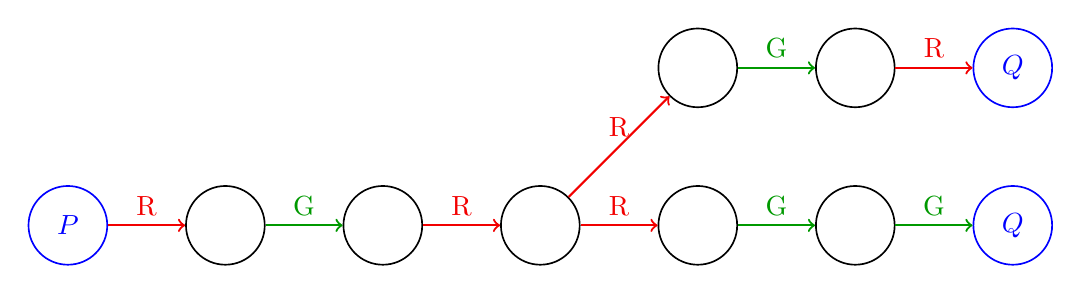
\begin{tikzpicture}[->, semithick]
\tikzset{
    prepost/.style= {circle, draw=blue, color=blue, minimum size=1.0cm},
    pstate/.style= {circle, draw=black, minimum size=1.0cm},
    prel/.style= {above, black!5!red, thick},
    pguar/.style= {above, black!40!green, thick},
}

\node[prepost] (P) at (0,0) {$P$};
\node[pstate] (s1) at (2,0) {};
\node[pstate] (s2) at (4,0) {};
\node[pstate] (s3) at (6,0) {};
\node[pstate] (s4) at (8,0) {};
\node[pstate] (s5) at (10,0) {};
\node[prepost] (s6) at (12,0) {$Q$};

\node[pstate] (s8) at (8,2) {};
\node[pstate] (s9) at (10,2) {};
\node[prepost] (s10) at (12,2) {$Q$};

\draw
(P) edge[prel] node {R} (s1)
(s1) edge[pguar] node {G} (s2)
(s2) edge[prel] node {R} (s3)
(s3) edge[prel] node {R} (s4)
(s4) edge[pguar] node {G} (s5)
(s5) edge[pguar] node {G} (s6)
(s3) edge[prel] node {R} (s8)
(s8) edge[pguar] node {G} (s9)
(s9) edge[prel] node {R} (s10);
\end{tikzpicture}
\captionof{figure}{An interleaving of environment and thread actions abstracted using rely/guarantee relations.}
\end{center}

A predicate $P$ that refers to the structure of a single state, describes a set of possible states, while binary relations represent a set of transitions that can happen in the system \cite{viktor}. The latter are predicates of the form $P_a(\vec{\sigma}, \sigma)$ that relate the state before action $a$ to the one right after. Given a single predicate we can define the two-state relation by placing no constraint on the old state, $P(\sigma) \triangleq P(\vec{\sigma}, \sigma)$ or on the other hand by not restricting the new state $\sigma$, $P(\vec{\sigma}) \triangleq P(\vec{\sigma}, \sigma)$. State relations can be sequentially composed in order to reflect the effect of actual program commands as follows $(P; Q)(\vec{\sigma}, \sigma) \triangleq \exists \alpha \ldotp P(\vec{\sigma}, \alpha) \land Q(\alpha, \sigma)$. We can now define that a binary relation $P$ is stable under another relation $Q$ if and only if $(P; Q) \Rightarrow P \land (Q; P) \Rightarrow P$ which means that whenever an action in $Q$ is done before or after a transition in $P$, this must not invalidate $P$ itself.

Every specification will now take the form $\triplena{R, G}{P}{C}{Q}$ and include the standard pre and postconditions, plus $R$ and $G$, the rely and guarantee relations. The rely relation models all actions that the environment can perform while the guarantee one describes what the thread executing $C$ has the ability to do. In order for the proof to be valid, $G$ needs to be stable under the interference of $R$. Stability is only explicitly checked at the atomic command level \cite{viktor} as the following inference rule describes.

\[
\infer[\textsc{RG-Atomic}]
{
	\triplena{R, G}{P}{\patomic{C}}{Q}
}
{
	\triplena{\mathsf{ID}, \top}{P}{C}{Q}
	\ \
	(P, Q) \in G
	\ \
	\pred{stable}{P, R}
	\ \
	\pred{stable}{Q, R}
}
\]

Given that $C$ executes atomically, there can be no interference from the environment, so $R \equiv \mathsf{ID}$, the identity relation, meaning that the state will be kept as it is. On the other hand, the guarantee relation $G \equiv \top$, allows any operation, although, as part of the premiss, we require the state pair $(P, Q)$ to be part of the original guarantee relation. The hard requirement is the explicit check of stability of $P$ and $Q$ under relation $R$.

\[
\infer[\textsc{RG-Par}]
{
	\triplena{R, G_1 \cup G_2}{P_1 \land P_2}{C_1\ ||\ C_2}{Q_1 \land Q_2}
}
{
	\triplena{R \cup G_2, G_1}{P_1}{C_1}{Q_1}
	\ \
	\triplena{R \cup G_1, G_2}{P_2}{C_2}{Q_2}
}
\]

Commands are composed in parallel using the \textsc{RG-Par} rule that makes the guarantee of the first command be part of the rely relation of the second one and vice-versa. This makes sure that we model all interference coming from concurrent threads.

\section{Modern Concurrent Reasoning}

The explanation of logic reasoning techniques continues by considering approaches that are currently used in concurrent systems. These frameworks allow to tackle the verification of heap-manipulating programs thanks to the advances brought by separation logic. Key results in this area have been achieved through the use of abstraction in specifications, which allows to use program logics in a client-module setting, and the formalisation of atomicity, a fundamental concept in concurrency where an operation is seen as happening in one single step.

\subsection{Hoare Logic}

As a starting point in proving correctness, or generally properties of computer programs, Hoare explains in \cite{hoare} how to use deductive reasoning in applying inference rules to a set of predefined language axioms. He specifies the use of what was later on referred to as a ``Hoare triple" of the shape $\triple{P}{C}{Q}$ where $P$ and $Q$ are first-order assertions while $C$ is the program executed. $P$ is called the precondition of $C$ while $Q$ is its postcondition. The triple thus describes that whenever the assertion $P$ holds before $C$ runs and at some point terminates, then $Q$ will hold on its completion. The kind of logic adopted, allows to reason about relatively simple programs involving integers and local variables living in the \textit{stack} of a function. Classic proofs performed using Hoare logic take the form of a proof tree with axioms as leaves and rules as intermediate steps. Such notation has the downside that complete proofs tend to explode in size. For this reason, proof sketches are utilized. They represent the holding assertions before and after every command that appears in the analyzed code. We can see an example of such in Figure \ref{fig:abshoare}.
\begin{gather*}
\begin{array}{l}
\specline{\top} \\
\pfunctions{abs}{\pvar{x}} \\
	\quad \passign{\pvar{r}}{\pvar{x}}; \\
	\quad \specline{\pvar{x} = \pvar{r}} \\
	\quad \pifelses{\pvar{x} < 0} \\
		\quad \quad \specline{\pvar{x} < 0 \land \pvar{x} = \pvar{r}} \\
		\quad \quad \passign{\pvar{r}}{-\pvar{x}}; \\
		\quad \quad \specline{\pvar{x} < 0 \land \pvar{r} = - \pvar{x}} \\
		\quad \quad \specline{(\pvar{x} < 0 \land \pvar{r} = -\pvar{x}) \lor (\pvar{x} \geq 0 \land \pvar{r} = \pvar{x})} \\
	\quad \pifelsem \\
		\quad \quad \specline{\pvar{x} \geq 0 \land \pvar{x} = \pvar{r}} \\
		\quad \quad \pskip; \\
		\quad \quad \specline{\pvar{x} \geq 0 \land \pvar{x} = \pvar{r}} \\
		\quad \quad \specline{(\pvar{x} < 0 \land \pvar{r} = -\pvar{x}) \lor (\pvar{x} \geq 0 \land \pvar{r} = \pvar{x})} \\
	\quad \pifelsee \\
	\quad \specline{(\pvar{x} < 0 \land \pvar{r} = -\pvar{x}) \lor (\pvar{x} \geq 0 \land \pvar{r} = \pvar{x})} \\
	\quad \preturn{\pvar{r}}; \\
\pfunctione \\
\specline{(\pvar{x} < 0 \land \pvar{ret} = -\pvar{x}) \lor (\pvar{x} \geq 0 \land \pvar{ret} = \pvar{x})} \\
\end{array}
\end{gather*}
\captionof{figure}{A proof sketch of the absolute value function using Hoare logic.}
\label{fig:abshoare} 

The $\mathtt{abs}(\pvar{x})$ function simply returns the absolute value of the input argument $\pvar{x}$. We notice that the procedure's precondition is $\top$ ($true$), which means that there is no particular assertion which needs to hold in order for the code to perform its task. On the other hand, the postcondition states that the return value, which is referred to using a special variable named $\pvar{ret}$, will effectively be the absolute value of $\pvar{x}$. Note how the postcondition of every command in a sequence becomes the precondition of the following one, respecting the rule specified in \cite{hoare}.

\subsection{Owicki-Gries}

In a concurrent setting, the first approach that allowed reasoning of programs was presented in \cite{owicki} and is referred to as the ``Owicki-Gries" method from the name of its authors. Its main contribution is the parallel composition rule.

\[
\infer[\textsc{Owicki-Gries}]
{\vdash \triple{P_1 \land P_2}{C_1\ ||\ C_2}{Q_1 \land Q_2}}
{\vdash \triple{P_1}{C_1}{Q_1} \ \vdash \triple{P_2}{C_2}{Q_2} \ \textsf{interference-free}}
\]

The rule states that we perform a regular sequential proof for each of the threads that are composed together and the resulting postcondition will be the conjunction of all the components' ones. This holds as long as the proofs of the individual thread runs are not interfering with each other. In other words, every intermediate assertion between atomic commands in the sequential proof of $C_1$ must be kept valid by the actions of $C_2$ and vice versa \cite{viktor}.
\[
\infer[\textsc{Cons}]
{
	\triple
	{\pvar{x} = 0}
	{\passign{\pvar{x}}{\pvar{x} + 1}\ ||\ \passign{\pvar{x}}{\pvar{x} + 2}}
	{\pvar{x} = 3}
}
{
	\infer[\textsc{Owicki-Gries}]
	{
		\triple
		{\pvar{x} = 0 \land \pvar{x} = 0}
		{\passign{\pvar{x}}{\pvar{x} + 1}\ ||\ \passign{\pvar{x}}{\pvar{x} + 2}}
		{(\pvar{x} = 1 \lor \pvar{x} = 3) \land (\pvar{x} = 2 \lor \pvar{x} = 3)}
	}
	{
		(\dag)
		\ \ \ \ \ \ \ \ \ \ \ \ \ \ \ \	
		(\spadesuit)
	}
}
\]

\[
(\dag) =
\infer[\textsc{Cons}]
		{
			\triple
			{\pvar{x} = 0}
			{\passign{\pvar{x}}{\pvar{x} + 1}}
			{\pvar{x} = 1 \lor \pvar{x} = 3}
		}
		{
			\infer[\textsc{Assign}]
			{
				\triple
				{\pvar{x} = 0 \lor \pvar{x} = 2}
				{\passign{\pvar{x}}{\pvar{x} + 1}}
				{\pvar{x} = 1 \lor \pvar{x} = 3}
			}
			{\ldots}		
		}
\]

\[
(\spadesuit) = 
\infer[\textsc{Cons}]
		{
			\triple
			{\pvar{x} = 0}
			{\passign{\pvar{x}}{\pvar{x} + 2}}
			{\pvar{x} = 2 \lor \pvar{x} = 3}
		}
		{
			\infer[\textsc{Assign}]
			{
				\triple
				{\pvar{x} = 0 \lor \pvar{x} = 1}
				{\passign{\pvar{x}}{\pvar{x} + 2}}
				{\pvar{x} = 2 \lor \pvar{x} = 3}
			}
			{\ldots}		
		}
\]

\[
\infer[\textsc{Cons}]
	{
		\triple
		{P}
		{C}
		{Q}
	}
	{
		P \Rightarrow P'\ \
		\triple
		{P'}
		{C}
		{Q'}\ \
		Q' \Rightarrow Q
	}
\]
\captionof{figure}{Partial proof tree of a parallel program incrementing variable $\pvar{x}$ which also uses the \textsc{Cons} rule (provided).}

The method's main burden is the \textsf{interference-free} constraint which makes non-trivial commands very complicated to prove. As a consequence, most specifications that satisfy the requirement will be too weak to prove any interesting properties about the concurrent code. This is the reason why such a method is only able to give stronger specifications using auxiliary or ghost variables whose task is to keep track of past program states. In addition, the actual code needs to be augmented with statements that refer to the ghost variables themselves. Any modular use of proofs that involve auxiliary variables would require new specifications, since the number of variables needed to express strong specifications would increase based on the way the module is used (e.g. the number of threads running). This becomes clear by looking at an example of two threads incrementing the same counter concurrently. We first define the counter's methods and then show a summarized proof \cite{modularsteps} of clients' usage through ghost variables.
\begin{gather*}
\begin{array}{@{}l@{\qquad}l@{\qquad}l@{}}
\begin{array}{@{}l@{}}
\pfunctions{makeCounter}{} \\
\quad \palloc{\pvar{c}}{1}; \\
\quad \pmutate{\pvar{c}}{0}; \\
\quad \preturn{\pvar{c}}; \\
\pfunctione
\end{array}
&
\begin{array}{@{}l@{}}
\pfunctions{increment}{\pvar{c}} \\
\quad \texttt{do } \{ \\
	\quad \quad \pderef{\pvar{n}}{\pvar{c}}; \\
	\quad \quad \pfuncall{\pvar{b}}{CAS}{\pvar{c}, \pvar{n}, \pvar{n} + 1}; \\
\quad \} \texttt{ while }(\pvar{b} = 0); \\
\quad \preturn{\pvar{n}}; \\
\pfunctione
\end{array}
\end{array} \\ \\
\pfuncall{\pvar{c}}{makeCounter}{};
\color{ForestGreen}\passign{\pvar{inc}_1}{0};
\passign{\pvar{inc}_2}{0}; \\
\color{blue} \{ \cell{\pvar{c}}{0} \land \pvar{inc}_1 = 0 \land \pvar{inc}_2 = 0 \} \\
\begin{array}{c || c}
\begin{array}{l}
\color{blue} \{ \cell{\pvar{c}}{\pvar{inc}_1 + \pvar{inc}_2} \land \pvar{inc}_1 = 0 \} \\
\texttt{do } \{ \\
	\quad \pderef{\pvar{n}}{\pvar{c}}; \\
	\quad \patomic{\pfuncall{\pvar{b}}{CAS}{\pvar{c}, \pvar{n}, \pvar{n} + 1}; \\
		\quad \quad \textcolor{ForestGreen}{\pifelses{\pvar{b}} \pvar{inc}_1\texttt{++}\pifelsee}} \\
\} \texttt{ while }(\pvar{b} = 0); \\
\color{blue} \{ \cell{\pvar{c}}{\pvar{inc}_1 + \pvar{inc}_2} \land \pvar{inc}_1 = 1 \} \\
\end{array}
&
\begin{array}{l}
\color{blue} \{ \cell{\pvar{c}}{\pvar{inc}_1 + \pvar{inc}_2} \land \pvar{inc}_2 = 0 \} \\
\texttt{do } \{ \\
	\quad \pderef{\pvar{n}'}{\pvar{c}}; \\
	\quad \patomic{\pfuncall{\pvar{b}'}{CAS}{\pvar{c}, \pvar{n}', \pvar{n}' + 1}; \\
		\quad \quad \textcolor{ForestGreen}{\pifelses{\pvar{b}'} \pvar{inc}_2\texttt{++}\pifelsee}} \\
\} \texttt{ while }(\pvar{b}' = 0); \\
\color{blue} \{ \cell{\pvar{c}}{\pvar{inc}_1 + \pvar{inc}_2} \land \pvar{inc}_2 = 1 \} \\
\end{array}
\end{array} \\
\color{blue} \{ \cell{\pvar{c}}{\pvar{inc}_1 + \pvar{inc}_2} \land \pvar{inc}_1 = 1 \land \pvar{inc}_2 = 1 \} \\
\color{blue} \{ \cell{\pvar{c}}{2} \}
\end{gather*}

As we can see, the parts of code in \textcolor{ForestGreen}{green} are auxiliary, i.e. they are not part of the executed code but are there to aid the proof. We use them to build the invariant that each of the two concurrent commands will use to prove its postcondition. In fact, at any point in the concurrent execution, the counter value will be the sum of the two auxiliary variables. Note that the increments to the ghost variables $\mathtt{inc}_1$ and $\mathtt{inc}_2$ must happen atomically with the respective $\mathtt{CAS}$ commands and this is the reason why they are included in an atomic context $\patomic{-}$.

If we now were to prove three separate threads incrementing the same counter in parallel, we would have to redo the proof, adding a new auxiliary variable $\mathtt{inc}_3$ and changing the invariants in all of the other bodies. The solution proposed is therefore not compositional. This implies that whenever we add a new method to a verified module which interacts with some shared state, we need to cross check every new command with all the others already present.

\subsection{Rely/Guarantee}

Jones \cite{jones} introduces a way of explicitly stating the interference coming from the environment as part of concurrent composition of code. This replaces the implicit and tedious side condition in the parallel rule of the ``Owicki-Gries" method. The result is rely/guarantee reasoning which is a compositional method. The specifications that arise from the use of such technique, adopt binary relations to express how the state might change as a result of the running thread's or the environment's actions.

\begin{center}
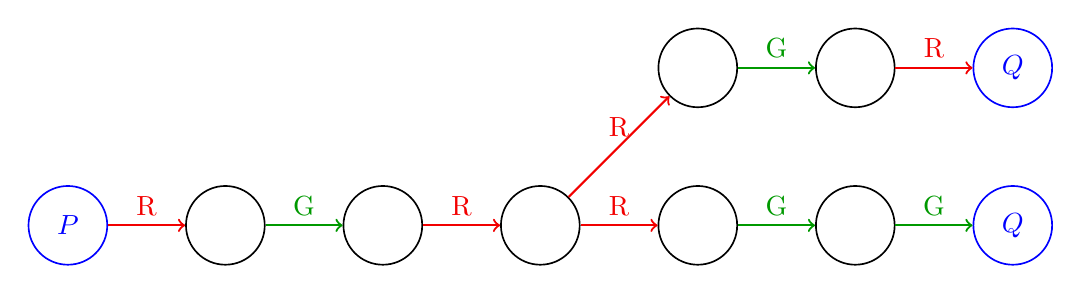
\begin{tikzpicture}[->, semithick]
\tikzset{
    prepost/.style= {circle, draw=blue, color=blue, minimum size=1.0cm},
    pstate/.style= {circle, draw=black, minimum size=1.0cm},
    prel/.style= {above, black!5!red, thick},
    pguar/.style= {above, black!40!green, thick},
}

\node[prepost] (P) at (0,0) {$P$};
\node[pstate] (s1) at (2,0) {};
\node[pstate] (s2) at (4,0) {};
\node[pstate] (s3) at (6,0) {};
\node[pstate] (s4) at (8,0) {};
\node[pstate] (s5) at (10,0) {};
\node[prepost] (s6) at (12,0) {$Q$};

\node[pstate] (s8) at (8,2) {};
\node[pstate] (s9) at (10,2) {};
\node[prepost] (s10) at (12,2) {$Q$};

\draw
(P) edge[prel] node {R} (s1)
(s1) edge[pguar] node {G} (s2)
(s2) edge[prel] node {R} (s3)
(s3) edge[prel] node {R} (s4)
(s4) edge[pguar] node {G} (s5)
(s5) edge[pguar] node {G} (s6)
(s3) edge[prel] node {R} (s8)
(s8) edge[pguar] node {G} (s9)
(s9) edge[prel] node {R} (s10);
\end{tikzpicture}
\captionof{figure}{An interleaving of environment and thread actions abstracted using rely/guarantee relations.}
\end{center}

A predicate $P$ that refers to the structure of a single state, describes a set of possible states, while binary relations represent a set of transitions that can happen in the system \cite{viktor}. The latter are predicates of the form $P_a(\vec{\sigma}, \sigma)$ that relate the state before action $a$ to the one right after. Given a single predicate we can define the two-state relation by placing no constraint on the old state, $P(\sigma) \triangleq P(\vec{\sigma}, \sigma)$ or on the other hand by not restricting the new state $\sigma$, $P(\vec{\sigma}) \triangleq P(\vec{\sigma}, \sigma)$. State relations can be sequentially composed in order to reflect the effect of actual program commands as follows $(P; Q)(\vec{\sigma}, \sigma) \triangleq \exists \alpha \ldotp P(\vec{\sigma}, \alpha) \land Q(\alpha, \sigma)$. We can now define that a binary relation $P$ is stable under another relation $Q$ if and only if $(P; Q) \Rightarrow P \land (Q; P) \Rightarrow P$ which means that whenever an action in $Q$ is done before or after a transition in $P$, this must not invalidate $P$ itself.

Every specification will now take the form $\triplena{R, G}{P}{C}{Q}$ and include the standard pre and postconditions, plus $R$ and $G$, the rely and guarantee relations. The rely relation models all actions that the environment can perform while the guarantee one describes what the thread executing $C$ has the ability to do. In order for the proof to be valid, $G$ needs to be stable under the interference of $R$. Stability is only explicitly checked at the atomic command level \cite{viktor} as the following inference rule describes.

\[
\infer[\textsc{RG-Atomic}]
{
	\triplena{R, G}{P}{\patomic{C}}{Q}
}
{
	\triplena{\mathsf{ID}, \top}{P}{C}{Q}
	\ \
	(P, Q) \in G
	\ \
	\pred{stable}{P, R}
	\ \
	\pred{stable}{Q, R}
}
\]

Given that $C$ executes atomically, there can be no interference from the environment, so $R \equiv \mathsf{ID}$, the identity relation, meaning that the state will be kept as it is. On the other hand, the guarantee relation $G \equiv \top$, allows any operation, although, as part of the premiss, we require the state pair $(P, Q)$ to be part of the original guarantee relation. The hard requirement is the explicit check of stability of $P$ and $Q$ under relation $R$.

\[
\infer[\textsc{RG-Par}]
{
	\triplena{R, G_1 \cup G_2}{P_1 \land P_2}{C_1\ ||\ C_2}{Q_1 \land Q_2}
}
{
	\triplena{R \cup G_2, G_1}{P_1}{C_1}{Q_1}
	\ \
	\triplena{R \cup G_1, G_2}{P_2}{C_2}{Q_2}
}
\]

Commands are composed in parallel using the \textsc{RG-Par} rule that makes the guarantee of the first command be part of the rely relation of the second one and vice-versa. This makes sure that we model all interference coming from concurrent threads.

\subsection{Concurrent Separation Logic}

In order to reason about heap manipulating programs, separation logic was introduced in \cite{seplogic} as a program logic which revolves around the concept of resource owning. The program state does not just involve values local to a method, but also ones that live in the shared \textit{heap} and that variables refer to through pointers. In terms of assertions, the main additions to Hoare's constructs are explained in the following list.
\begin{itemize}
\item The separating conjunction $P \lstar Q$ asserts that the state can be divided into two disjoint parts, one of which satisfies predicate $P$ and the other one $Q$.
\item $\cell{E_1}{E_2}$ asserts that there exists a memory cell whose address can be obtained by evaluating $E_1$ and whose value is $E_2$.
\item The empty assertion $emp$ states that the \textit{heap} must contain no allocated cells.
\end{itemize}

The separating conjunction empowers the program logic to have a frame rule which allows to prove a specification by temporarily not considering additional resources in the heap that are not accessed as part of the command we are verifying.

\[
\infer[\textsc{Frame}]
{\vdash \triple{P \lstar R}{C}{Q \lstar R}}
{\vdash \triple{P}{C}{Q} \ \ \pred{mod}{C} \cap \pred{fv}{R} \equiv \emptyset}
\]

The requirement for it to work, is that no variable which is modified as part of running command $C$ can be free in predicate $R$. Another way of looking at the rule is that if we are able to prove a triple, then adding an arbitrary resource, which is not touched by the command, will not invalidate our original proof. In later work \cite{csl}, O'Hearn included support for disjoint concurrency through a new rule.
\begin{gather*}
\infer[\textsc{SL-Par}]
{\vdash \triple{P_1 \lstar P_2}{C_1\ ||\ C_2}{Q_1 \lstar Q_2}}
{\vdash \triple{P_1}{C_1}{Q_1} \ \vdash \triple{P_2}{C_2}{Q_2} \ \pred{nc}{C_1, C_2, P_2, Q_2} \ \pred{nc}{C_2, C_1, P_1, Q_1}}
\\
\pred{nc}{C, C', P, Q} \triangleq \pred{mod}{C} \cap (\pred{fv}{C'} \cup \pred{fv}{P} \cup \pred{fv}{Q}) \equiv \emptyset
\end{gather*}

The rule states that as long as two threads only access disjoint parts of memory to execute, then they can safely be composed in parallel. The disjointness requirement appears as a side-condition to the rule, expressed through the non conflict predicate $\mathsf{nc}$.

\subsection{RGSep} \label{rgsep}

The efforts developed as part of separation logic and rely/guarantee reasoning were brought together by RGSep \cite{viktor}. Its main contribution was related to the separation between the local state $l$ and shared one $s$. In an abstract sense, $l$ and $s$ are members of a resource algebra $(M, \odot, \mathsf{u})$ such that $l \odot s$ is defined if and only if the two are disjoint. In the latter case, the entirety of the state is defined to be the union of $l$ and $s$. In order to distinguish them, a new kind of assertion, the shared assertion, is introduced and often referred to as the ``boxed assertion". In fact, $\boxed{P}$ expresses a generic separation logic assertion $P$ which refers to the shared state $s$. The separating conjunction $\lstar$ works in the usual way inside of the local state but behaves additively for the shared one. As a consequence we have that $\boxed{P} \lstar \boxed{Q} \Leftrightarrow \boxed{P \land Q}$.

Interference between parallel threads is modelled using actions of the form $P \transto Q$. The action meaning is that the part of the shared state where $P$ holds will be replaced with a part that satisfies $Q$ leaving the rest of $s$ intact. For example, if we were describing the action that allows to increment a counter stored at address $x$, we would have something along the lines of $\cell{x}{n} \transto \cell{x, m} \land m \geq n$.

RGSep requires all preconditions and postconditions of commands in a proof to be stable under interference coming from the environment. We can syntactically check for stability as follows.
\begin{align*}
\pred{stable}{S, \sem{P \transto Q}} &\Leftrightarrow\ \vDash ((P \sepimp S) \lstar Q) \Rightarrow S
\\
\pred{stable}{S, (R_1 \cup R_2)^*} &\Leftrightarrow\ \vDash \pred{stable}{S, R_1} \land \pred{stable}{S, R_2}
\end{align*}
The first property states that if we take a state $S$ and remove the part satisfying $P$ and add one where $Q$ holds then $S$ will hold again. On the other hand, the second property defines that a statement is stable with respect to a set of actions when it is stable under the interference of every action in the set. Given that actions can only affect the shared state $s$, the stability check only needs to be performed on assertions which refer to $s$ itself.

\subsection{CAP}

The program logic explained in \cite{cap} makes use of separation logic constructs to allow abstraction on shared data structures using concurrent abstract predicates. These provide a disjointness of shared resources at the abstraction level which might not be reflected in the actual implementation. For example, if we consider a set module and formulate a predicate stating that ``the set is $\{ 1,2 \}$", then we want to remove element $2$ and be able to assert that the set is now $\{ 1 \}$. In order to reason about the module in such a fine-grained manner, we want element $2$ to be manipulated independently from the rest of the set. This kind of disjointness expressed at the level of abstraction does not need to be part of the implementation. In fact one could implement the set module using a singly linked list which requires traversing some elements before reaching the desired item.

Concurrent abstract predicates also hold information regarding what kind of interference is allowed on the shared memory from the thread and the environment. Fractional permissions \cite{fractional} are utilized in order to model the type of control a thread has on a particular shared structure. On top of this, implementation code can be formally verified against high level specifications and later be \textit{hidden} to clients that make use of it by allowing them not to refer to low-level details in their own proof derivations.

Standard separation logic is augmented with two novel assertions, the shared region and the permission one. The first takes the shape $\sharedr{P}$ and represents a part of memory, associated with an identifier $r$, which is shared among several threads and satisfies predicate $P$. The region is indivisible so that all threads accessing it always get a consistent view of it; we can enforce such behaviour as $\sharedr{P} \lstar \sharedr{Q} \Leftrightarrow \sharedr{P \land Q}$. The permission assertion $[\tguard{A}]_\pi^r$ gives the thread the possibility to perform action $\tguard{A}$ on region $r$ with fractional permission $\pi$. The latter will be a real value in $(0, 1)$ when both the thread and the environment can execute $\tguard{A}$ or equals to $1$ in the case where the thread is the only one to be able to do so. We can combine permissions to perform the same action in the same region in the following way, $[\tguard{A}]_{\pi_1}^r \lstar [\tguard{A}]_{\pi_2}^r \Leftrightarrow [\tguard{A}]_{\pi_1 + \pi_2}^r$. Actions in CAP are similar to the ones seen in Section \ref{rgsep} and have the form $\tguard{A}: P \transto Q$ where the label is followed by two assertions that describe the part of the region needed for $\tguard{A}$ and the same part after the action has taken place. All possible actions for a particular region $r$ are summarized inside $I(r, \vec{x})$. We can create a shared region from a predicate $P \Rrightarrow \exists r \ldotp \sharedr{P} \lstar \pred{all}{I(r, \vec{x})}$ by including every action permission available.

We now have all the ingredients to prove the specification \cite{cap} of a lock module in CAP. The latter will provide three methods, namely \texttt{makeLock()}, \texttt{lock(x)} and \texttt{unlock(x)}. As the names suggest, the first method will allocate the necessary resources for a lock and initiate it while the other two will acquire or release the lock at address $\pvar{x}$. Following these English specifications we can provide formal ones.
\begin{gather*}
\triple
{emp}
{\mathtt{makeLock}()}
{\exists x \ldotp \pvar{ret} = x \land \pred{isLock}{x} \lstar \pred{Locked}{x}}
\\
\triple
{\pred{isLock}{\pvar{x}}}
{\mathtt{lock}(\pvar{x})}
{\pred{isLock}{\pvar{x}} \lstar \pred{Locked}{\pvar{x}}}
\\
\triple
{\pred{Locked}{\pvar{x}}}
{\mathtt{unlock}(\pvar{x})}
{emp}
\end{gather*}

The actions allowed on the lock are $\tguard{L}$ and $\tguard{U}$ which are used to interpret the abstract predicates used in the specification.
\begin{align*}
\pred{isLock}{x} &\equiv \exists r, \pi \ldotp [\tguard{L}]_\pi^r \lstar \sharedrs{(\cell{x}{0} \lstar [\tguard{U}]_1^r) \lor \cell{x}{1}}
\\
\pred{Locked}{x} &\equiv \exists r \ldotp [\tguard{U}]_1^r \lstar \sharedrs{\cell{x}{1}}
\\
I(r, x) &\triangleq 
\left\lbrace
\begin{array}{rl}
\tguard{L}: & [\tguard{U}]_1^r \lstar \cell{x}{0} \transto \cell{x}{1} \\
\tguard{U}: & \cell{x}{1} \transto [\tguard{U}]_1^r \lstar \cell{x}{0}
\end{array}
\right\rbrace
\end{align*}

The $\pred{isLock}{x}$ predicate gives a thread knowledge of the existence of a lock at address $x$ which can either be in the locked or unlocked state based on the value $x$ points to. It also provides a permission to perform the $\tguard{L}$ action to acquire the lock. Given the nature of the predicate we can state that $\pred{isLock}{x} \Rightarrow \pred{isLock}{x} \lstar \pred{isLock}{x}$ holds as we are simply sharing the knowledge of $x$ being a lock.

On the other hand, $\pred{Locked}{x}$ describes that the lock at $x$ is currently locked and has been previously acquired by the thread that holds the predicate. As the $\pred{Locked}{x}$ predicate gives us full permission of $[\tguard{U}]_1^r$, we have that $\pred{Locked}{x} \lstar \pred{Locked}{x} \Rightarrow \bot$ since a thread cannot acquire the lock twice sequentially. Action $\tguard{L}$'s effect requires the lock to be unlocked and for the region to include the permission to perform $\tguard{U}$. In fact, once the action is performed, the latter permission will be removed from the region and included in the thread's local state so that no other thread can release the lock. $\tguard{U}$ has instead the opposite behaviour: it requires the lock to be acquired and once done, it will put the unlock permission back in the shared region. The specification provided will be used to verify a concrete implementation of the lock module using a spin lock whose code is given in Figure \ref{fig:spinlock}.

\begin{figure}
\[
\begin{array}{@{}l@{\qquad}l@{\qquad}l@{}}
\begin{array}{@{}l@{}}
\pfunctions{lock}{\pvar{x}} \\
	\quad \mathtt{do}\ \{ \\
		\quad \quad \pfuncall{\pvar{b}}{CAS}{\pvar{x}, 0, 1}; \\
	\quad \}\ \mathtt{while}\ (\pvar{b} = 0); \\
\pfunctione
\end{array}
&
\begin{array}{@{}l@{}}
\pfunctions{unlock}{\pvar{x}} \\
	\quad \patomic{\pmutate{\pvar{x}}{0}}; \\
\pfunctione
\end{array}
&
\begin{array}{@{}l@{}}
\pfunctions{makeLock}{} \\
	\quad \palloc{\pvar{x}}{1}; \\
	\quad \pmutate{\pvar{x}}{1}; \\
	\quad \preturn{\pvar{x}}; \\
\pfunctione
\end{array}
\end{array}
\]
\captionof{figure}{A spin lock implementation using \texttt{CAS}.}
\label{fig:spinlock}
\end{figure}

The \texttt{lock} method uses a popular mechanism to handle synchronization, namely compare-and-swap. \texttt{CAS}($a$, $c$, $v$) works by atomically comparing the dereferenced value of $a$ with $c$ and in case of a match, $a$ is set to point to $v$. In case of a successful swap, \texttt{CAS} returns 1, otherwise it returns 0.

\begin{figure}
\[
\begin{array}{l}
\specline{\pred{isLock}{\pvar{x}}} \\
\pfunctions{lock}{\pvar{x}} \\
	\quad \specline{\exists r, \pi \ldotp [\tguard{L}]_\pi^r \lstar \sharedrs{(\cell{\pvar{x}}{0} \lstar [\tguard{U}]_1^r) \lor \cell{\pvar{x}}{1}}} \\
	\quad \mathtt{do}\ \{ \\
		\quad \quad \pfuncall{\pvar{b}}{CAS}{\pvar{x}, 0, 1}; \\
		\quad \quad \specline{\exists r, \pi \ldotp \left( [\tguard{L}]_\pi^r \lstar \sharedrs{(\cell{\pvar{x}}{0} \lstar [\tguard{U}]_1^r) \lor \cell{\pvar{x}}{1}} \land \pvar{b} = 0 \right) \\ \lor \left( [\tguard{L}]_\pi^r \lstar [\tguard{U}]_1^r \lstar \sharedr{\cell{\pvar{x}}{1}} \land \pvar{b} = 1 \right)} \\
	\quad \}\ \mathtt{while}\ (\pvar{b} = 0); \\
	\quad \specline{[\tguard{L}]_\pi^r \lstar [\tguard{U}]_1^r \lstar \sharedr{\cell{\pvar{x}}{1}}} \\
\pfunctione \\
\specline{\pred{isLock}{\pvar{x}} \lstar \pred{Locked}{\pvar{x}}}
\end{array}
\]
\captionof{figure}{The spin lock's \texttt{lock} function implementation proof.}
\label{fig:spinproof}
\end{figure}

In Figure \ref{fig:spinproof} we give a CAP sketch proof of the \texttt{lock(x)} method which is shown to satisfy its specification. Note how the use of \texttt{CAS} is combined with a while loop whose condition is the outcome of the swap. This way we can be sure that once the control flow of the program exits the loop, the lock's state is updated and the $\tguard{L}$ action has taken place.

\subsection{Abstract atomicity and Linearizability}

We refer to an operation as atomic when it happens at a single discrete point in time \cite{modularsteps}. Whenever atomic actions are performed concurrently, the actual execution will always be an interleaving of those. In general, even if a command is built from multiple operations, abstract atomicity can be obtained if the overall effect appears to be atomic.

Linearizability \cite{linearizability} is a correctness condition which allows methods of a concurrent module to be used by clients as atomic. All of such module operations are provided with sequential specifications that are proven to behave atomically with respect to each other. As a consequence, the moment a new method is added to the module, the linearizability proof for all methods needs to be performed. The main contribution of the approach is the fact that specifications that guarantee linearizability are an abstraction which can be directly used by clients of the module to reason without having to worry about the implementation details.

\subsection{TaDA} \label{s:tada}

TaDA \cite{tada} is a modern program logic that combines the perks of the CAP approach and of linearizability to allow modular proofs of concurrent programs. Its main novelty is the introduction of atomic specifications as a first-order construct through the use of atomic triples. These have the form $\atriplenl{}{x \in X}{P(x)}{C}{Q(x)}$ and indicate that command $C$ will atomically update the state from $P$ to $Q$ in a single, discrete step.

\begin{center}
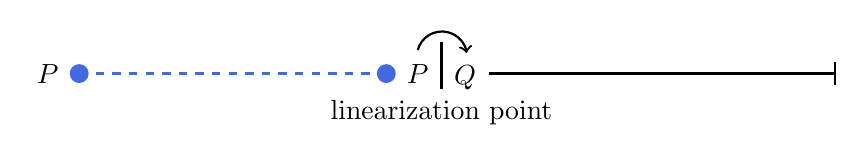
\begin{tikzpicture}[thick]
\node (Ps) at (0, 0) {$P$};
\node (P) at (4.7, 0) {$P$};
\node (Q) at (5.3, -0.05) {$Q$};
\node (L) at (5, -0.5) {linearization point};

\filldraw[color=RoyalBlue] (0.4, 0) circle (3pt);
\filldraw[color=RoyalBlue] (4.3, 0) circle (3pt);
\draw[color=RoyalBlue, dashed] (0.4, 0) -- (4.3, 0);
\draw (5, 0.4) -- (5, -0.2);
\draw (5.6, 0) -- (10, 0);
\draw (10, 0.15) -- (10, -0.15);
\draw [->] (4.7, 0.3) arc (165:8:9pt); 
\end{tikzpicture}
\end{center}

More specifically, the triple actually states that, due to the environment's interference, the variable bound by the pseudo-quantifier $\aall$ (in this case $x$) can vary within the values of set $X$ as long as it still satisfies precondition $P(x)$. Then, right at the function's linearization point, the $C$ command will atomically bring the state to satisfy $Q(x)$. After this, the command does not give any guarantees on the validity of $Q(x)$ since it might be changed by another thread running concurrently. On the other hand, $C$ will not change the state of $x$ again after the linearization point but it can use it to refer to its value right before the event. The specifications give a notion of atomicity which is only maintained at the level of abstraction defined by $P$. In fact, observing the state at a lower level might show several distinct steps involved as part of the command.

We will explore TaDA's rules and constructs while going through a concrete program example of a stack data structure module, which supports concurrent access. The concurrent stack module will have a simple interface for clients to use that allows the creation of a new stack and the ability to push and pop items from it.

Note that the full atomic triple has the shape $\atriplee{}{x \in X}{P_p}{P(x)}{C}{y \in Y}{Q_p(x, y)}{Q(x, y)}$ where the first part of the state is private to the thread. This includes all assertions which are stable under the environment's intereference. Everything which is instead on the public side of the state, accepts interference as described by the guarded transitions for regions. Whenever we encounter a standard Hoare triple $\triple{P}{C}{Q}$ in TaDA, we can see it as pure syntactic sugar for $\atriplenq{}{P}{\top}{C}{Q}{\top}$ where there is effectively no public state.	
\begin{gather*}
\triple{emp}{\mathtt{makeStack}()}{\exists r \ldotp \pred{S}{r, \pvar{ret}, []}}
\\
\atriplenl
{}
{l}
{\pred{S}{r, \pvar{x}, l} \land \pvar{v} \neq 0}
{\pfuncallnr{push}{\pvar{x}, \pvar{v}}}
{\pred{S}{r, \pvar{x}, \pvar{v}\cons l}}
\\
\vatriplenl
{}
{l}
{\pred{S}{r, \pvar{x}, l}}
{\mathtt{pop}(\pvar{x})}
{(\pred{S}{r, \pvar{x}, []} \land \pvar{ret} = 0) \lor (\exists l'\ldotp \pred{S}{r, \pvar{x}, l'} \land l = \pvar{ret}\cons l' \land \pvar{ret} \neq 0)}
\end{gather*}

The \texttt{makeStack()} method is given a sequential specification, since it would be unreal to use a shared structure during its creation. In a more likely setup, a single thread creates the stack and then passes its reference to other (potentially child) threads. The function's return value will be a pointer to the new data structure. Adding elements to the stack is done through the use of \texttt{push}(\texttt{x},\texttt{v}) which puts the item \texttt{v} on top of the stack. We require an atomic specification for the method as the environment might interact with the structure while we are pushing to it. The inserted value must be different from $0$ due to the fact that the return value of \texttt{pop(x)} will be $0$ in the case of an empty stack. This is just a simplified convention, given the abscence of error handling in this demonstrating example. The abstract predicate $\pred{S}{r, x, l}$, in a style similar to CAP, indicates the presence of a stack in the shared region identified by $r$, at memory address $x$ with contents $l$. We can formally define it as follows.
\begin{align*}
\pred{S}{r, x, l} \triangleq &\exists h, ns, ds \ldotp \textbf{Stack}_r(x, h, ns, ds) \lstar [\tguard{G}]_r \land l = \pred{values}{ns}
\\
\text{where } &\pred{values}{[]} \triangleq []
\\
&\pred{values}{(-, v) \cons l} \triangleq v \cons \pred{values}{l}
\end{align*}

The $\textbf{Stack}_r(x, h, ns, ds)$ predicate is a region type describing the structure of a shared region in memory. In addition to that, $[\tguard{G}]_r$ is a guard that is associated to the region as an abstract resource. It gives a thread the permission to perform action $\tguard{G}$ on shared region $r$. Actions in TaDA are defined inside a labelled transition system that maps guards to possible updates to the region. In our case, we express a single guard which gives the ability to both push and pop from the stack. In the second case, the update actually only happens when the stack is non-empty.
\begin{align*}
&\tguard{G}: \forall n, v \neq 0, ns, ds \ldotp (ns, ds) \transto ((n, v) \cons ns, ds)
\\
&\tguard{G}: \forall n, v, ns, ds \ldotp (ns, ds) \transto \ite{ns = (n, v) \cons ns'}{(ns', (n, v) \cons ds)}{(ns, ds)}
\end{align*}

We unveil the meaning of the additional arguments of $\textbf{Stack}_r$ by providing a region interpretation for the latter.
\begin{align*}
I(\textbf{Stack}_r(x, h, ns, ds)) \triangleq &\cell{x}{h} \lstar \mathsf{stack}(h, ns) \lstar \bigoast_{(n, v) \in ds} \twocell{n}{v}{-}
\\
\text{where } &\mathsf{stack}(h, []) \triangleq h = \snull
\\
&\mathsf{stack}(h, (h, v) \cons l) \triangleq v \neq 0 \land \exists z . \twocell{h}{v}{z} \lstar \mathsf{stack}(z, l)
\end{align*}

The stack's address $x$ points to the head node, $h$, which is the first node of the structure that will be either $\snull$ for an empty stack or point to a value and a subsequent node. On top of this, $ns$ is a logical list including all active node pairs $(n, v)$ in the stack where $n$ is the node's address and $v$ the value it points to. Those nodes that were at one point part of the stack but have been popped since, are called dead nodes and included in the set $ds$. As we can see from the transition system, every time an item is popped, it is virtually moved from $ns$ to $ds$ to keep track of it. This additional information, which can be seen as a ghost state of the program, is particularly helpful when proving the \texttt{pop} function implementation. In fact, if the function pops an item $n$ which has been concurrently removed since we first read it, then it is necessary to know that it had the $\twocell{n}{-}{-}$ structure and this information is provided as part of the dead nodes assertion.

\begin{figure}[h]
\[
	\begin{array}{l}
		\pfunction{\pvar{makeStack}}
		{}
		{
		\\
		\quad \palloc{\pvar{x}}{1};
		\\
		\quad \preturn{\pvar{x}}; \\
		}
		\end{array}
		\ \ \ \
		\begin{array}{l}
		\pfunction{\pvar{push}}
		{\pvar{x}, \pvar{v}}
		{
		\\
		\quad \palloc{\pvar{fst}}{2};
		\\
		\quad \pmutate{\pvar{fst}}{\pvar{v}};
		\\
		\\
		\quad \mathtt{do} \ \{
		\\
		\quad \quad \pderef{\pvar{h}}{\pvar{x}};
		\\
		\quad \quad \pmutate{\pvar{fst} + 1}{\pvar{h}};
		\\
		\quad \quad \pfuncall{\pvar{b}}{CAS}{\pvar{x}, \pvar{h}, \pvar{fst}};
		\\
		\quad\} \ \mathtt{while}\ (\pvar{b} = 0);
		\\
		}
		\end{array}
		\ \ \ \
		\begin{array}{l}
		\pfunction{\pvar{pop}}
		{\pvar{x}}
		{
		\\
		\quad \passign{\pvar{r}}{0};
		\\
		\quad \mathtt{do} \ \{
		\\
		\quad \quad \passign{\pvar{b}}{0};
		\\
		\quad \quad \pderef{\pvar{h}}{\pvar{x}};
		\\
		\quad\quad \pifelses{\pvar{h} = \snull}
		\\
		\quad\quad \quad \preturn{0};
		\\
		\quad\quad \pifelsem
		\\
		\quad \quad \quad \pderef{\pvar{r}}{\pvar{h}};
		\\
		\quad \quad \quad \pderef{\pvar{next}}{\pvar{h} + 1};
		\\
		\quad \quad \quad \pfuncall{\pvar{b}}{CAS}{\pvar{x}, \pvar{h}, \pvar{next}};
		\\
		\quad\quad \pifelsee
		\\
		\quad\} \ \mathtt{while}\ (\pvar{b} = 0);
		\\
		\\
		\quad \preturn{\pvar{r}};
		\\
		}
	\end{array}
	\label{fig:concurrentstack}
	\]
	\captionof{figure}{The concurrent stack \textsc{While} language implementation with the addition of the compare-and-swap (\texttt{CAS}) command.}
\end{figure}

We provide an implementation of the three methods in Figure \ref{fig:concurrentstack} followed by a full TaDA proof of the $\pfuncallnr{push}{\pvar{x}, \pvar{v}}$ function. The proof begins by unwrapping the $\pred{S}{r, \pvar{x}, l}$ abstract predicate into its definition which includes the $\textbf{Stack}_r$ region predicate and the $[\tguard{G}]_r$  action guard. We use the latter as part of the \textsc{MakeAtomic} rule, in order to modify the underlying stack structure to insert a new element, $\pvar{v}$. This step gives us the atomicity tracking component $\atomtok$ and the ability of treating a sequence of commands as if they happened atomically. As part of the function's body, we allocate memory for the node (\texttt{fst}) that will host the new element and begin a loop whose task is to read the stack's head node into \texttt{h} and use \texttt{CAS} to atomically set it to \texttt{fst} only when \texttt{h} is equivalent to $[\pvar{x}]$ (meaning that the value of the stack's head has not changed since we first read it into \texttt{h}). We prove all of this using the following inference rules:
\begin{itemize}
\item \textsc{Existential} in order to get rid of the existential quantifiers on logical variables $h, ns, ds$ and to be able to apply the next rules.
\item The \textsc{AWeakening} rule to turn the logical variables $h, ns, ds$ into pseudo-quantified ones (bound by $\aall$) and to prove an atomic triple referring to the update that follows.
\item \textsc{UpdateRegion} consumes the atomicity tracking component to try and update the shared region $\textbf{Stack}_r$ by first opening it up and revealing its interpretation. Later, the update can either succeed or fail, as described by the rule's postcondition that includes a disjunction.
\item We \textsc{Frame} out all assertions only leaving $\cell{\pvar{x}}{h}$ since this is all we need to conclude the proof. In fact, the $\pfuncallnr{CAS}{\pvar{x}, \pvar{h}, \pvar{fst}}$ command does not modify any other variables a part from $\pvar{x}$.
\item The \textsc{CAS} rule finally allows us to condition the actual update on the boolean return value, $\pvar{b}$ which is used inside the following postconditions to understand whether the swap has happened or not.
\end{itemize}

\newgeometry{margin=2cm}
\[
\small{
\begin{array}{l}
	\quantifierline{\aall l \ldotp} \\
	\aspecline{\pred{S}{r, \pvar{x}, l} \land \pvar{v} \neq 0} \\
	\pfunction{\pvar{push}}{\pvar{x}, \pvar{v}}{ \\
		\quad \aspecline{\pred{S}{r, \pvar{x}, l} \land \pvar{v} \neq 0} \\
		\quad \begin{leftvruled}{abstract}
			\aspecline{\exists h, ns, ds \ldotp \textbf{Stack}_r(\pvar{x}, h, ns, ds) \lstar [\tguard{G}]_r \land l = \pred{values}{ns} \land \pvar{v} \neq 0} \\
			\begin{leftvruled}{atomic exists on $ns$, $ds$}
				\quantifierline{\aall ns, ds \ldotp} \\
				\aspecline{\exists h \ldotp \textbf{Stack}_r(\pvar{x}, h, ns, ds) \lstar [\tguard{G}]_r \land l = \pred{values}{ns} \land \pvar{v} \neq 0} \\
				\begin{leftvruled}{make atomic}
					\acontextline{r : (ns, ds) \transto ((-, \pvar{v}) \cons ns, ds) \land \pvar{v} \neq 0 \vdash} \\
					\specline{\exists h, ns, ds \ldotp \textbf{Stack}_r(\pvar{x}, h, ns, ds) \land l = \pred{values}{ns} \lstar r \Mapsto \atomtok \land \pvar{v} \neq 0} \\
					\palloc{\pvar{fst}}{2}; \pmutate{\pvar{fst}}{\pvar{l}}; \\
					\specline{\exists h, ns, ds \ldotp \textbf{Stack}_r(\pvar{x}, h, ns, ds) \land l = \pred{values}{ns} \lstar r \Mapsto \atomtok \lstar \twocell{\pvar{fst}}{\pvar{v}}{\snull} \land \pvar{v} \neq 0} \\
					\mathtt{do} \ \{ \\
						\quad \specline{\exists h, ns, ds, s \ldotp \textbf{Stack}_r(\pvar{x}, h, ns, ds) \land l = \pred{values}{ns} \lstar r \Mapsto \atomtok \lstar \twocell{\pvar{fst}}{\pvar{v}}{s} \land \pvar{v} \neq 0} \\
						\quad \begin{leftvruled}{open region}
							\quantifierline{\aall h, ns, ds \ldotp}
							\aspecline{\cell{\pvar{x}}{h} \lstar \mathsf{stack}(h, ns) \lstar \bigoast_{(n, v) \in ds} \twocell{n}{v}{-}} \\
							\begin{leftvruled}{frame}
								\quantifierline{\aall h \ldotp} \aspecline{\cell{\pvar{x}}{h}} \\
								\pderef{\pvar{h}}{\pvar{x}}; \\
								\aspecline{\cell{\pvar{x}}{h} \land \pvar{h} = h}
							\quad \end{leftvruled} \\
							\aspecline{\cell{\pvar{x}}{h} \lstar \mathsf{stack}(h, ns) \lstar \bigoast_{(n, v) \in ds} \twocell{n}{v}{-} \land \pvar{h} = h} \\
						\end{leftvruled} \\
						\quad \specline{\exists h, ns, ds, s, a \ldotp \textbf{Stack}_r(\pvar{x}, h, ns, ds) \land l = \pred{values}{ns} \lstar r \Mapsto \atomtok \lstar \twocell{\pvar{fst}}{\pvar{v}}{s} \land \pvar{h} = a \land \pvar{v} \neq 0} \\
						\quad \pmutate{\pvar{fst} + 1}{\pvar{h}}; \\
						\quad \specline{\exists h, ns, ds \ldotp \textbf{Stack}_r(\pvar{x}, h, ns, ds) \land l = \pred{values}{ns} \lstar r \Mapsto \atomtok \lstar \twocell{\pvar{fst}}{\pvar{v}}{\pvar{h}} \land \pvar{v} \neq 0} \\
						\quad \begin{leftvruled}{existential on $h, ns, ds$}
							\specline{\textbf{Stack}_r(\pvar{x}, h, ns, ds) \land l = \pred{values}{ns} \lstar r \Mapsto \atomtok \lstar \twocell{\pvar{fst}}{\pvar{v}}{\pvar{h}} \land \pvar{v} \neq 0} \\
							\begin{leftvruled}{weakening on $h$, $ns$, $ds$}
								\quantifierline{\aall h, ns, ds \ldotp} \\
								\aspecline{\textbf{Stack}_r(\pvar{x}, h, ns, ds) \land l = \pred{values}{ns} \lstar r \Mapsto \atomtok \lstar \twocell{\pvar{fst}}{\pvar{v}}{\pvar{h}} \land \pvar{v} \neq 0} \\
								\begin{leftvruled}{update region}
									\aspecline{\cell{\pvar{x}}{h} \lstar \mathsf{stack}(h, ns) \lstar \bigoast_{(n, v) \in ds} \twocell{n}{v}{-} \land l = \pred{values}{ns} \lstar \twocell{\pvar{fst}}{\pvar{v}}{\pvar{h}} \land \pvar{v} \neq 0} \\
									\begin{leftvruled}{frame, CAS}
										\quantifierline{\aall h \ldotp} \\
										\aspecline{\cell{\pvar{x}}{h}} \\
										\pfuncall{\pvar{b}}{CAS}{\pvar{x}, \pvar{h}, \pvar{fst}}; \\
										\aspecline{(\pvar{b} = 0 \land \cell{\pvar{x}}{h} \land \pvar{h} \neq h)
										\lor (\pvar{b} = 1 \land \cell{\pvar{x}}{\pvar{fst}} \land \pvar{h} = h)}
									\end{leftvruled} \\
									\aspecline{(\pvar{b} = 0 \land \pvar{h} \neq h \land \cell{\pvar{x}}{h} \lstar
									\mathsf{stack}(h, ns) \lstar \twocell{\pvar{fst}}{\pvar{v}}{\pvar{h}}) \\
									\lor (\pvar{b} = 1 \land \pvar{h} = h \land \cell{\pvar{x}}{\pvar{fst}} \lstar
									\twocell{\pvar{fst}}{\pvar{v}}{\pvar{h}} \lstar \mathsf{stack}(\pvar{h}, ns)) \\
									\lstar \bigoast_{(n, v) \in ds} \twocell{n}{v}{-} \land l = \pred{values}{ns} \land \pvar{v} \neq 0}
								\end{leftvruled} \\
								\aspecline{l = \pred{values}{ns} \land \pvar{v} \neq 0 \land ((\pvar{b} = 0 \land \textbf{Stack}_r(\pvar{x}, h, ns, ds) \lstar \twocell{\pvar{fst}}{\pvar{v}}{\pvar{h}} \lstar r \Mapsto \atomtok) \\
								\lor (\pvar{b} = 1 \land \textbf{Stack}_r(\pvar{x}, h, (\pvar{fst}, \pvar{v}) \cons ns, ds)) \lstar r \Mapsto ((ns, ds), ((-, \pvar{v}) \cons ns, ds)))}
							\end{leftvruled} \\
							\specline{((\pvar{b} = 0 \land \textbf{Stack}_r(\pvar{x}, h, ns, ds) \lstar \twocell{\pvar{fst}}{\pvar{v}}{\pvar{h}} \lstar r \Mapsto \atomtok) \\ \lor (\pvar{b} = 1 \lstar r \Mapsto ((ns, ds), ((-, \pvar{v}) \cons ns, ds))) \land l = \pred{values}{ns} \land \pvar{v} \neq 0}
						\end{leftvruled} \\
						\quad \specline{\exists h, ns, ds \ldotp ((\pvar{b} = 0 \land
						\textbf{Stack}_r(\pvar{x}, h, ns, ds) \lstar \twocell{\pvar{fst}}{\pvar{v}}{\pvar{h}}
						\lstar r \Mapsto \atomtok) \\
						\lor (\pvar{b} = 1 \lstar r \Mapsto ((ns, ds), ((-, \pvar{v}) \cons ns, ds)))  \land l = \pred{values}{ns} \land \pvar{v} \neq 0} \\
					\} \ \mathtt{while}(\pvar{b} = 0); \\
					\specline{\exists h, ns, ds \ldotp l = \pred{values}{ns} \lstar r \Mapsto ((ns, ds), ((-, \pvar{v}) \cons ns, ds))} \\
				\end{leftvruled} \\
				\aspecline{\exists h \ldotp \textbf{Stack}_r(\pvar{x}, h, (-, \pvar{v}) \cons ns, ds) \lstar [\tguard{G}]_r \land l = \pred{values}{ns}} \\
			\end{leftvruled} \\
			\aspecline{\exists h, ns, ds \ldotp \textbf{Stack}_r(\pvar{x}, h, (-, \pvar{v}) \cons ns, ds) \lstar [\tguard{G}]_r \land l = \pred{values}{ns}} \\
		\end{leftvruled} \\
		\quad \aspecline{\pred{S}{r, \pvar{x}, \pvar{v}\cons l}} \\
	}
\end{array}
}
\]
\restoregeometry

As part of the logic, there are some key inference rules that are displayed in the \texttt{push} proof. For an exhaustive list and explanation we point the reader to \cite{tada}. First of all, \textsc{MakeAtomic} allows to take an atomic specification and prove the abstract atomicity of a sequence of non-atomic commands where a single linearization point will appear and update the shared state. In order to do so, we must hold the guard of the appropriate action for the region. In the premiss, we obtain the atomicity tracker component in the form of an abstract resource ($\atomtok$). This works like a token used to recognize whether the atomic update declared in the atomicity context ($\acontextline{a : x \transto f(x)}$) has already happened or not. On a successful update, the token will be converted into the state transition described by the guarded action. As we can see from the postcondition of the premiss, the atomic update \textit{must} happen at some point in order to satisfy the rule.
\begin{gather*}
f : X \rightarrow Y \ \ \left\lbrace (x, y)\ |\ x \in X, y \in f(x) \right\rbrace \subseteq \mathcal{T}_\textbf{t}^* \\
\infer
{
\atriplenl
	{}
	{x \in X}
	{\textbf{t}_a(\vec{z}, x) \lstar [\tguard{G}]_a}
	{C}
	{\exists y \in f(x) \ldotp \textbf{t}_a(\vec{z}, y) \lstar [\tguard{G}]_a}
}
{
\triplena
	{\acontextline{a : x \in X \transto f(x)}}
	{\exists x \in X \ldotp \textbf{t}_a(\vec{z}, x) \lstar a \Mapsto \atomtok}
	{C}
	{\exists x \in X, y \in f(x) \ldotp a \Mapsto (x, y)}
}
\\
\textsc{MakeAtomic}
\end{gather*}

The moment we need to access the contents of a shared region to unveil its interpretation, we can use one of two rules: \textsc{OpenRegion} and \textsc{UpdateRegion}. The first one allows to view the underlying content of a region but it forbids any update to its abstract state. For this reason, it neither needs an explicit guard nor a tracking component to be used. On the other hand the \textsc{UpdateRegion} rule is employed to perform the atomic update of the region's abstract state. It requires the update not to have happened already and we can guarantee that with the presence of the atomicity token in the precondition. Inside the postcondition we need to take into account whether the update has succeeded or not and we do that by having a disjunction on the two possible predicates that hold for the region.
\begin{gather*}
\infer
{
\atriplenl
{\acontextline{a : x \in X \transto f(x)}}
{x \in X}
{\textbf{t}_a(\vec{z}, x) \lstar P(x) \\
	\lstar a \Mapsto \atomtok}
{C}
{\exists y \in f(x) \ldotp \textbf{t}_a(\vec{z}, y) \\ \lstar Q_1(x, y) \lstar
		a \Mapsto (x, y) \lor \\ \textbf{t}_a(\vec{z}, x) \lstar Q_2(x) \lstar a \Mapsto \atomtok}
}
{
\atriplenl
	{}
	{x \in X}
	{I(\textbf{t}_a(\vec{z}, x)) \lstar P(x)}
	{C}
	{\exists y \in f(x) \ldotp I(\textbf{t}_a(\vec{z}, y)) \lstar Q_1(x, y) \\
		\lor I(\textbf{t}_a(\vec{z}, x)) \lstar Q_2(x)}
}
\\
\textsc{UpdateRegion}
\end{gather*}

Another way to update a shared region is to apply the \textsc{UseAtomic} rule which grants the permission to perform such change through an explicit guard held in the precondition, in contrast with the atomicity tracking component in \textsc{UpdateRegion}. The use of this inference rule implies that command $C$ acts atomically at an abstraction level which is lower than the one of region $a$ and as a consequence, it will be atomic at the higher level as well. This way we can stack a layer of abstraction on top of another which gives a lot of flexibility in terms of writing program modules that extend or make use of other pre-verified modules.
\begin{gather*}
f : X \rightarrow Y \ \ \left\lbrace (x, y)\ |\ x \in X, y \in f(x) \right\rbrace \subseteq \mathcal{T}_\textbf{t}^* \\
\infer
{
\atriplenl
{}
{x \in X}
{\textbf{t}_a(\vec{z}, x) \lstar [\tguard{G}]_a}
{C}
{\exists y \in f(x) \ldotp \textbf{t}_a(\vec{z}, y) \lstar [\tguard{G}]_a}
}
{
\atriplenl
{}
{x \in X}
{I(\textbf{t}_a(\vec{z}, x)) \lstar [\tguard{G}]_a}
{C}
{\exists y \in f(x) \ldotp I(\textbf{t}_a(\vec{z}, y)) \lstar [\tguard{G}]_a}
}
\\
\textsc{UseAtomic}
\end{gather*}

Finally, the \textsc{Frame} rule works in the same way as in separation logic, by adding resources to the precondition and postcondition of a command that does not modify them. As we can notice in the \texttt{push} proof, we can also frame out predicates referring to variables bound by $\aall$.
\begin{gather*}
\pred{mod}{C} \cap \pred{vars}{R_p} \equiv \emptyset\ \
\pred{mod}{C} \cap \pred{vars}{R(x)} \equiv \emptyset \\
\infer
{
	\atriple
	{}
	{x \in X}
	{P_p \lstar R_p}
	{P(x) \lstar R(x)}
	{C}
	{Q_p(x, y) \lstar R_p}
	{Q(x, y) \lstar R(x)}
}
{
	\atriplee
	{}
	{x \in X}
	{P_p}
	{P(x)}
	{C}
	{y \in Y}
	{Q_p(x, y)}
	{Q(x, y)}
}
\\
\textsc{Frame}
\end{gather*}

\section{Database Theory}

This section shifts the focus from program logics to the main theory behind a database. This is generically abstracted from a particular instantiation, which enables us to describe its properties from a high-level point of view, without considering its implementation. We are mainly interested in the concurrent aspects of modern databases, therefore we concentrate on transactions and the way they are managed.

\tocless\subsection{Transactions}

A database is a collection of data items that hold values. A database system (\textit{DBS}) is a tool comprised of software and hardware components that manages access to the underlying database. It allows its users to perform specific operations on the database items. Those can be summarized as being one of two kinds, reads and writes. In the following, we will use the notation \tread{x} to represent a read operation of the database item named \textit{x} while \twrite{x}{v} to depict a write operation which sets item \textit{x}'s value to \textit{v}. We will use the shorthand notation \twritee{x} to mean that some value is written to item $x$. Both the mentioned kind of operations are executed atomically \cite{ccontrol}. This means that the execution of a set of such operations appears to be sequential in terms of its constituents.

It is often the case that several operations are grouped together in order to make them behave as if they were a single unit of work. In such situations, database transactions are used: an ordered collection of operations. For example, considering a database for bank accounts, we consider a transfer of funds as a single operation from the user's point of view even if in reality the \textit{DBS} performs multiple sequential reads and writes to achieve the goal, as shown in Figure \ref{fig:transfer}. A transaction execution must provide guarantees on the well known \textbf{ACID} properties \cite{dbconcepts}, an acronym for:
\begin{enumerate}[ref=(\arabic*)]
\item \label{acid.a} Atomicity: all of the transaction's operations are executed or none of them; there is no possible partial execution of a transaction.
\item \label{acid.c} Consistency: an isolated execution of a transaction maintains the consistency constraints of the database. In our bank example, the property would be maintained when money is neither created nor destroyed as part of a transfer, but simply \textit{moved}.
\item \label{acid.i} Isolation: a transaction executes as if no other one is running in the \textit{DBS} at the same time. More generally, a given isolation level determines the correct behaviours of transactions that run concurrently. For example, serializability implies that any two transactions running in parallel believe that the other one has either finished before they started or it will start after they finished executing.
\item \label{acid.d} Durability: once a transaction has completed its work, all of its changes are kept in the database even if failures happen in the future.
\end{enumerate}

In order to maintain property \ref{acid.a}, a transaction needs to communicate the completion of its operations or its interruption in case of failure. This is done by introducing two new types of operation, namely commit and abort, which are notated \tcommit and \tabort respectively. In the case of an abort, the \textit{DBS} must roll-back the state of the database to what it was prior to the start of the transaction in order to undo the changes performed up to the failure point.

\begin{center}
\begin{tabular}{c@{\hskip 0.5in}c}
\begin{lstlisting}
BEGIN
	balance := R[a]
	W[a, balance-100]
	balance := R[b]
	W[b, balance+100]
	C
END
\end{lstlisting}
&
\begin{lstlisting}
BEGIN
	balance := R[a]
	W[a, balance-5000]
	A
END
\end{lstlisting}
\end{tabular}
\captionof{figure}{Two examples of transactions on the bank database. Note how the second one aborts due to a failure (potentially insufficient funds).}
\label{fig:transfer}
\end{center}

Following the explanation in \cite{ccontrol}, we formally define a transaction $T$ as the tuple $(\theta, \sqsubset)$ where $\theta$ is the set of all operations in $T$ and $\sqsubset$ is a partial order on $\theta$. The latter is defined as:
\[
	\theta \subseteq \left\lbrace op\ |\ op \in \lbrace \tread{x}^i, \twritee{x}^i \rbrace, x \in \pred{items}{db}, i \in \mathds{N} \right\rbrace \cup \left\lbrace \tcommit, \tabort \right\rbrace
\]
The set of operations, $\theta$, maintains the constraint $\left(\tcommit \in \theta \Leftrightarrow \tabort \notin \theta\right)$ while the ordering relation, $\sqsubset$, must satisfy the property that if the transaction contains an operation $t$ which is either a commit or an abort, then all operations must appear in a transaction before $t$. Formally,
\[
	\forall t \in \{\tcommit, \tabort\} \ldotp t \in \theta \Rightarrow \left( \forall op \in \theta \ldotp op \neq t \Rightarrow op \sqsubset t \right)
\]

Also, we state that, as part of a single transaction, any two operations that involve a particular item, with at least one of them being a write, must be ordered according to $\sqsubset$:
\begin{gather*}
	\forall x \in \pred{items}{db}, op, i, j \ldotp \left( op \in \left\lbrace \tread{x}^i, \twritee{x}^i \right\rbrace \land \lbrace op, \twritee{x}^j \rbrace \subseteq \theta \land i \neq j \right) \\ \implies (\twritee{x}^j \sqsubset op \lor op \sqsubset \twritee{x}^j)
\end{gather*}
For the example in Figure \ref{fig:transfer} we would have the following transaction definition:
\begin{gather*}
\theta \equiv \left\lbrace \tmread{\texttt{a}}^1, \tmread{\texttt{b}}^2, \tmwritee{\texttt{a}}^3, \tmwritee{\texttt{b}}^4, \tcommit \right\rbrace
\\[0.4em]
\sqsubset\ \equiv \{ (\tmread{\texttt{a}}^1, \tmwritee{\texttt{a}}^3), (\tmread{\texttt{b}}^2, \tmwritee{\texttt{b}}^4), (\tmread{\texttt{a}}^1, \tcommit), (\tmread{\texttt{b}}^2, \tcommit), (\tmwritee{\texttt{a}}^3, \tcommit), (\tmwritee{\texttt{b}}^4, \tcommit) \}
\end{gather*}
This gives the \textit{DBS} the option to arbitrarily schedule the operations which are not ordered according to $\sqsubset$. In fact, under the mentioned example, one could invert the order of the two reads (or even run them in parallel) and still always get to the same final result. As we will see in section \ref{histories}, if a history is proven to be serializable, then we can guarantee valuable properties about it.

\tocless\subsection{Histories} \label{histories}

Modern database systems employ concurrency in order to run multiple transactions at the same time to achieve a higher performance and better operations throughput. On the downside, running operations in parallel on shared data items can lead to race conditions and a potential loss of two of the aforementioned ACID properties, consistency and isolation.

% In order to investigate the matter further, we will introduce some definitions which will prove useful.
The interleaving of operations which arises from a concurrent run of transactions, is referred to as a history. It records the order in which operations actually happen on the database and given that some of them could effectively execute in parallel, they are not totally ordered. A history $H$ \cite{ccontrol} is therefore a tuple $(\Theta, \pord)$ such that for a set of $n$ transactions $T_H = \left\lbrace T_i \right\rbrace_{i \in I}$, where $I = \{ i\ |\ 1 \leq i \leq n\}$, we have the operations set $\Theta$ and the partial order $\pord$ such that:
\[
	\begin{array}{c}
		\Theta \triangleq \bigcup_{i = 1}^{n} \theta_i\
		\text{ and }\
		\bigcup_{i = 1}^{n} \sqsubset_i\ \subseteq \pord
	\end{array}
\]
When inside a history, single operations are tagged with the transaction they belong to, e.g. $\tread{x}^n_i$ refers to a read with identifier $n$ performed on item $x$ by transaction $i$. Whenever we omit the superscript and the subscript, we assume that they are implicitly existentially quantified.

Let's now define two operations as conflicting if they both access the same data item and one of them is a write; formally we describe the property as:
\begin{gather*}
	\pred{conflict}{op_\alpha, op_\beta} \\
	\iff \\
	op_\alpha \neq op_\beta \land \left(\left( op_\alpha \in \{ \tread{x}, \twritee{x} \} \land op_\beta = \twritee{x} \right) \lor \left( op_\alpha = \twritee{x} \land op_\beta \in \{ \tread{x}, \twritee{x} \} \right)\right)
\end{gather*}
We then require that all conflicting operations appearing in a history must be somehow ordered by $\pord$.
\[
	\forall op_\alpha, op_\beta \ldotp (\pred{conflict}{op_\alpha, op_\beta} \land\left\lbrace op_\alpha, op_\beta \right\rbrace \subseteq \Theta) \Rightarrow (op_\alpha \pord op_\beta \lor op_\beta \pord op_\alpha)
\]
When considering a history $H_{total}$ which is a total order over the operations of its transactions, we can refer to it simply by $\twritee{x}_i^1, $ $\twritee{y}_j^1, $ $\tcommit_i, $ $\tread{x}_j^2, $ $\twritee{x}_j^3, $ $\tcommit_j$ for example.

For every history $H = (\Theta, \pord)$ we can compute the group of transactions which committed as part of it as the set:
\[
	\pred{committed}{H} \triangleq \{ T_i\ |\ \tcommit_i \in \Theta \}
\]
This definition will aid us in describing a fundamental structure for the analysis of histories, the precedence or serialization graph. The latter allows to establish relationships between the transactions committing their operations as part a history. We can now build a history's precedence graph $G(H) = (V, E)$ where the set of vertices $V = \pred{committed}{H}$ includes all committed transactions in $H$ and an edge $(T_i, T_j)$ is in $E$, if transaction $T_i$ has an operation which is ordered before one in $T_j$ and the two are conflicting \cite{dbconcepts}. Formally, the set of edges is defined as:
\[
	E \triangleq \{ (T_i, T_j)\ |\ i \neq j \land \exists op_\alpha, op_\beta \ldotp op_\alpha \in \theta_i \land op_\beta \in \theta_j \land op_\alpha\ \pord\ op_\beta \land \pred{conflict}{op_\alpha, op_\beta} \}
\]

In Figure \ref{fig:exPrecGraph} we can see a concrete instance of a history with $3$ transactions and its corresponding precedence graph. Note that the graph's nodes include the three transactions since they all commit as part of $H$. On top of this, the edge from $T_1$ to $T_2$ is justified by pair the conflicting operations $(\tmread{x}_1^1, \tmwritee{x}_2^2)$, while the one from $T_1$ to $T_2$ by the pair $(\tmread{y}_1^2, \tmwritee{y}_3^1)$.\\

\begin{center}
\begin{tikzpicture}[->, semithick]
\node (1) {$T_1$};
\node (2) [right = 0.5cm of 1] {$T_2$};
\node (3) [right = 0.5cm of 2] {$T_3$};

\path
(1) edge node {} (2)
(1) edge [bend left] node {} (3);
\end{tikzpicture}
\\[0.4em]
$H \equiv \tmread{x}_1^1, \tmread{x}_2^1, \tmread{y}_1^2, \tmwritee{x}_2^2, \tcommit_2, \tmwritee{y}_3^1, \tcommit_1, \tcommit_3$
\captionof{figure}{An example history with its corresponding precedence graph.}
\label{fig:exPrecGraph}
\end{center}

A history $H_i$ is said to be equivalent to another history $H_j$ \cite{ccontrol}, when they have the same set of transactions which committed as part of them, and they order conflicting operations in the same way. We formally write $H_i \equiv H_j$, and this holds if and only if:
\begin{gather*}
	\pred{committed}{H_i} \equiv \pred{committed}{H_j} \\
	\land \forall op_\alpha, op_\beta \ldotp (\pred{conflict}{op_\alpha, op_\beta} \land \left\lbrace op_\alpha, op_\beta \right\rbrace \subseteq \Theta_i) \Rightarrow (op_\alpha\ \pord_i\ op_\beta \Leftrightarrow op_\alpha\ \pord_j\ op_\beta)
\end{gather*}
The latter condition is necessary because the result of a concurrent execution of a set of transactions only depends upon the relative ordering of conflicting operations. We describe a history as serial if all of its constituent transactions are run one after the other, without an interleaving of their operations. Such histories guarantee the highest possible database isolation. It is possible to further state that any history $H$ is serializable if and only if it is equivalent to some serial history $H'$. The serializability theorem states that any history $H$, such that its precedence graph $G(H)$ contains no cycles, is serializable \cite{ccontrol}.

\tocless\subsection{Anomalies and Isolation Levels}

The \textsc{Ansi/Iso Sql-92} standard \cite{ansi92} defines a set of different transaction isolation levels based on partial histories they allow as part of the possible interleavings. We will call these sequences of actions phenomena. The original standard describes 3 of such phenomena, while Berenson et al. \cite{isolationansi} add an extra one \ref{ansi:0} for completeness. \\

\begin{enumerate}[label=(\textbf{P\arabic*})]\addtocounter{enumi}{-1}
\item \label{ansi:0} A \textbf{dirty write} appears when a transaction $T_i$ writes to a data item and, before it commits or aborts, another transaction $T_j$ writes to the same item. If any of $T_i$ and $T_j$ were to abort, it is not clear what value the item should contain.
\\
E.g. $H_{DW} \equiv \ldots \tmwritee{x}_i \ldots \tmwritee{x}_j \ldots$
\item We have the \textbf{dirty read} phenomenon in the case where transaction $T_i$ writes to an item, then, before it commits or aborts, another transaction $T_j$ reads that same data item. In fact if $T_i$ would abort after $T_j$ has already read, the latter would have retrieved a value for the item that never actually existed.
\\
E.g. $H_{DR} \equiv \ldots \twritee{x}_i \ldots \tread{x}_j \ldots$
\item A \textbf{non-repeatable read} happens when a transaction $T_i$ reads a data item which is later written to by another transaction $T_j$ that also commits. At this point, if $T_i$ is to read the same item again, it would either discover a new value or fail due to a removal.
\\
E.g. $H_{NR} \equiv \ldots \tread{x}_i \ldots \twritee{x}_j \ldots \tcommit_j \ldots$
\item The \textbf{phantom} phenomenon appears when transaction $T_i$ queries all data items satisfying a particular condition $\gamma$. Transaction $T_j$ then inserts some new items that satisfy $\gamma$. Now, if $T_i$ were to reproduce the initial query, it would see new items appear.
\\
E.g. $H_{P} \equiv \ldots \tmread{\gamma}_i \ldots \tmwritee{\gamma}_j \ldots \tmread{\gamma}_i \ldots$ here we abuse the transaction notation in the following way $\tmread{\gamma} \triangleq \left\lbrace x\ |\ x \in \pred{items}{db} \land \gamma(x) \right\rbrace$ and $\tmwritee{\gamma} \triangleq \exists x, v \ldotp \gamma(x) \land \tmwrite{x}{v}$.
\end{enumerate}

The listed definitions can be used to formulate the \textsc{Ansi} isolation levels as they appear in Table \ref{table:isolation}. The choice of how to concurrently run several transactions given by a $DBS$ allows clients to achieve a better performance or stronger consistency depending on how strict the isolation level is. In fact, allowing some of the phenomena can lead to failing constraint checks in the database.
\begin{center}
\captionof{table}{\textsc{Ansi} isolation levels and the phenomena they allow \cite{ansi92} \cite{isolationansi}.}
\def\arraystretch{1.4}
	\begin{tabular}{l|c c c c}
		\hline
		\textbf{Isolation Level} & \textbf{Dirty Write} & \textbf{Dirty Read} & \textbf{N-R Read} & \textbf{Phantom} \\
		\hline
		Read Uncommitted & $\times$ & \checkmark & \checkmark & \checkmark \\
		Read Committed & $\times$ & $\times$ & \checkmark & \checkmark \\
		Repeatable Read & $\times$ & $\times$ & $\times$ & \checkmark \\
		Serializable & $\times$ & $\times$ & $\times$ & $\times$ \\
		\hline
	\end{tabular}
\label{table:isolation}
\end{center}

A concrete example of how the presence of the described phenomena can lead to a lack of correctness is shown in Table \ref{table:inconsistent} where transactions run at the read committed level. Let's assume that $T_i$ is executed by a bank's agent that wants to read what percentage of the overall funds are held by customer $a$ and $T_j$ is directly performed by $a$ as a cash withdrawal from an ATM machine. The former would first read the balance of $a$ then sum the funds of all customers (in this case $a$, $b$, $c$) and perform a simple division. On the other hand, $T_j$ will first read the cash availability, then subtract $\$100$ and provide the money to the customer. Given the isolation level selected, a non-repeatable read appears as part of history $H$ as $T_j$ removes the money after $T_i$ has read the initial balance for $a$ and before it has computed the overall sum. Therefore the end result $(\texttt{b}\div\texttt{total})$ will be incorrect and larger than the actual one. Moreover, this is a consequence to the fact that $H$ is not serializable. We can show this by first noticing that there are two possible serial histories:
\begin{align*}
	H_1 &= \tmread{a}_1^1, \tmread{a}_1^2, \tmread{b}_1^3, \tmread{c}_1^4, \tcommit_1, \tmread{a}_2^1, \tmwritee{a}_2^2, \tcommit_2 \\[0.5em]
	H_2 &= \tmread{a}_2^1, \tmwritee{a}_2^2, \tcommit_2, \tmread{a}_1^1, \tmread{a}_1^2, \tmread{b}_1^3, \tmread{c}_1^4, \tcommit_1
\end{align*}
The conflicting operations that happen as part of the execution are the pairs $(\tmread{a}_1^1, \tmwritee{a}_2^2)$ and $(\tmread{a}_1^2, \tmwritee{a}_2^2)$. The relative order in which they appear in the histories we consider is expressed as follows:
\[
	\begin{array}{c}
		H: \tmread{a}_1^1\ \pord_H\ \tmwritee{a}_2^2\ \pord_H\ \tmread{a}_1^2
		\\[0.5em]
		\begin{array}{c c}
			H_1 : \tmread{a}_1^1\ \pord_{H_1}\ \tmread{a}_1^2\ \pord_{H_1}\ \tmwritee{a}_2^2\
			&\
			H_2 : \tmwritee{a}_2^2\ \pord_{H_2}\ \tmread{a}_1^1\ \pord_{H_2}\ \tmread{a}_1^2
		\end{array}
	\end{array}
\]
It is clear that the particular ordering of conflicts in $H$ is neither the same as the one in $H_1$, nor to the one in $H_2$. Therefore since $H$ is not equivalent to any of $H_1$ and $H_2$, it is clearly not serializable. A plausible solution for this kind of issue is to change the isolation level of the $DBS$ to repeatable read which forbids the presence of the culprit phenomenon.
\begin{center}
\captionof{table}{History $H$ showing a concurrent run of two transactions $T_i$ and $T_j$.}
\def\arraystretch{1.4}
\begin{tabular}{c|@{\hspace{15pt}} c @{\hspace{15pt}} c}
\hline
\textbf{Time $t$} & $T_i$ & $T_j$ \\
\hline
0 & \texttt{b} = $\tmread{a}_i^1$ & \texttt{c} = $\tmread{a}_j^1$ \\
1 & - & $\tmwrite{a}{\texttt{c}-100}_j^2$ \\
2 & - & \tcommit \\
3 & \texttt{total} = $\tmread{a}_i^2$ + $\tmread{b}_i^3$ + $\tmread{c}_i^4$ & - \\
4 & \tcommit & - \\
\hline
\end{tabular}
\label{table:inconsistent}
\end{center}

\tocless\subsection{Locking Protocols}

The most popular mechanism to enforce a particular isolation level is to use some form of locking. We can consider each data item $x \in \pred{items}{db}$ to be associated with a lock that manages the access to its value. When a transaction runs an operation which accesses $x$, it is required to hold the lock relative to the item. The exact synchronization structure used in this case is a read/write lock that works under two modes, a shared one and an exclusive one. The former allows multiple read operations to happen in parallel while the latter makes sure that there is only one write operation executing at any point in time. This way, execution blocking only happens when transactions perform concurrent conflicting operations on the same data item. In terms of notation, a transaction $T_i$ can lock an item using $\tlock{\kappa}{x}_i$ and unlock it with $\tunlock{\kappa}{x}_i$ where $\kappa \in \{ \tshared, \texclusive \}$ is the lock mode (shared or exclusive). If a transaction requests access to item $x$ and gets an immediate grant even if $x$'s lock is held by another transaction, we say that the two locks are compatible \cite{dbconcepts}. We define this property for lock modes as follows:
\[
	\pred{compatible}{\kappa, \kappa'} \iff (\kappa = \tshared \land \kappa' = \tshared)
\]

We can specify the usage of locks in a formal way by describing histories $H$ that arise from locking protocols. Given that all accesses to database items are well locked, we know that they must be guarded by the corresponding and appropriate locks which are later released, so:
\begin{gather*}
	\forall x, i \ldotp \left( \tmwritee{x}_i \in \Theta_H \implies \tlock{\texclusive}{x}_i\ \pord\ \tmwritee{x}_i\ \pord\ \tunlock{\texclusive}{x}_i \right) \\[0.3em]
	\land \left( \tmread{x}_i \in \Theta_H \implies \exists \kappa \ldotp \tlock{\kappa}{x}_i\ \pord\ \tmread{x}_i\ \pord\ \tunlock{\kappa}{x}_i \right)
\end{gather*}
On top of this, when that a transaction requests an already acquired and non-compatible lock, it must wait for the counterpart to release. This implies that as part of locking protocols' histories, we will see that:
\begin{gather*}
	\forall x, \kappa_a, \kappa_b, i, j \ldotp \\
	(i \neq j \land \lnot \pred{compatible}{\kappa_a, \kappa_b} \land \{ \tlock{\kappa_a}{x}_i, \tunlock{\kappa_a}{x}_i, \tlock{\kappa_b}{x}_j, \tunlock{\kappa_b}{x}_j \}\subseteq \Theta_H) \\
	 \implies (\tunlock{\kappa_b}{x}_j\ \pord\ \tlock{\kappa_a}{x}_i \lor \tunlock{\kappa_a}{x}_i\ \pord\ \tlock{\kappa_b}{x}_j)
\end{gather*}

Two-Phase-Locking (\tpl) is a concurrency control protocol which is vastly used in commercial $DBS$ products. In its base version, as the name suggests, each transaction $T_i$'s execution can be divided into two phases \cite{ccontrol}: a growing phase where $T_i$ sequentially acquires locks for all the data items it is going to access, and a shrinking phase that starts on the first lock release and will unlock all the items it holds, one after the other. According to \tpl, during the growing phase no locks are released, and once the shrinking phase has started, no locks are acquired. Formally, all histories that result from the use of \tpl\ will have an additional property in comparison to the ones already mentioned for locking protocols. In fact lock operations will be further ordered as to comply with the two phase separation:
\[
	\forall x, y, \kappa_a, \kappa_b, i \ldotp (\{ \tlock{\kappa_a}{x}_i, \tunlock{\kappa_b}{y}_i \} \subset \Theta_H \implies \tlock{\kappa_a}{x}_i\ \pord\ \tunlock{\kappa_b}{y}_i)
\]

A variation of the method is Conservative Two-Phase-Locking (\textsc{c2pl}) that works in a similar way with the key difference that all locks ever needed as part of a transaction are acquired before any read or write operation happens. As a consequence, we can state that all histories $H$ adhering to \textsc{c2pl} will be such that:
\[
	\forall x, op, \kappa, i \ldotp (op \neq \textsf{L} \land \{ \tlock{\kappa}{x}_i, op \} \subseteq \Theta_H) \Rightarrow \tlock{\kappa}{x}_i\ \pord\ op
\]
This is done primarily in order to prevent situations in which \tpl\ would exhibit deadlocks, since lock acquisitions can be done in some precise order that all transactions need to follow.

Another version of \tpl\ which is widely used inside concrete implementations is Strict Two-Phase-Locking (\stpl) which imposes a different kind of constraint. Specifically, it only allows transactions to release the locks they hold after they have either committed or aborted. Its histories follow the rules listed for standard \tpl\ and moreover they guarantee that:
\[
	\forall x, op, \kappa, i \ldotp (op \in \{ \tcommit_i, \tabort_i \} \land \{ \tunlock{\kappa}{x}_i, op \} \subset \Theta_H) \Rightarrow op\ \pord\ \tunlock{\kappa}{x}_i
\]
The Strong-Strict Two-Phase-Locking (\textsc{ss2pl}) protocol works by combining the two previous approaches in a way that all locking operations happen before any access to items and all unlocking operations appear after a transaction's commit or abort completion. We summarize the pecularities of the four variants of the protocol in Table \ref{table:2plvariants}. Gradual locking refers to a transaction acquiring locks for cells as it needs to, while the extreme version makes it obtain all needed locks before starting. Similarly, gradual unlocking releases locks whenever they are no longer needed (while still following the two phases rule) and, on the other hand, extreme unlocking only releases locks after a transaction has committed.
\begin{center}
\captionof{table}{Two-Phase-Locking variants' constraints.}
\setlength{\tabcolsep}{14pt}
\def\arraystretch{1.6}
\begin{tabular}{l|c c c c}
\hline
\textbf{Constraint} & \textsc{2pl} & \textsc{c2pl} & \textsc{s2pl} & \textsc{ss2pl} \\
\hline
Gradual Locking & \checkmark & $\times$ & \checkmark & $\times$ \\
Extreme Locking & $\times$ & \checkmark & $\times$ & \checkmark \\
Gradual Unlocking & \checkmark & \checkmark & $\times$ & $\times$ \\
Extreme Unlocking & $\times$ & $\times$ & \checkmark & \checkmark \\
\hline
\end{tabular}
\label{table:2plvariants}
\end{center}

\tocless\subsection{Serializability \& Transactional Models}

\label{sec:serTransMod}

The theory for database transactions that we introduced so far has recently had a large number of applications to the more general context of programming languages. Transactions are being effectively used in the latter to provide an overall simplification to shared-memory concurrency. Popular commercial programming languages provide syntactic constructs to embed a chunk of code into an atomic transaction. This allows to free programmers from the burden of mantaining the fictional atomicity of operations, and delegate everything to the language implementation. We explore two models of transactions in this setting. On top of this, we later explain work related to reasoning about consistency models within distributed databases. \\

\paragraph{Push/Pull Model}
The model of transactions described in \cite{pushPull} is presented as a general theory of serializability, that abstracts away all of the algorithm and implementation details, in order to find a compact set of operations used in the vast majority of cases. The model does not use a concrete machine state, i.e. a global storage or memory heap, to track the effect of transactions' operations such as writes. Instead, it assigns a local \textit{log} of operations to each transaction and considers a unique shared log, which records the history of all globally visible operations. The semantics allow transactions to \textsc{Push} or \textsc{Unpush}, in order to share their local effects with the global log or to recall them from it. Conversely, they can \textsc{Pull} an operation from the shared log into their local view, together with detangling from one through an \textsc{Unpull}. These two types of actions can be seen as reading or \textit{forgetting} a read from the global storage. The framework comes with a proof of serializability within the semantic model, meaning that once users map their algorithms to the \textit{Push/Pull} semantic rules, they obtain a proof of serializability as a consequence.

\paragraph{Semantics for Transactions} The work done in \cite{semanticsTransactions} presents a set of formal languages which are able to describe particular behaviours that arise from the use of transactions within a programming language. Those are defined in terms of small-step operational semantics that allow the interleaving of parallel operations. They are high-level in order not to appear too complicated to the eyes of a programmer, while still detailed enough to express the required features. The languages of the \textsf{AtomsFamily} are listed here, in increasing order of consistency strictness:
\begin{enumerate}
	\item \label{highLevel.1} As part of \textsf{StrongBasic} only one single thread is allowed to execute a transaction at one time. On top of this, a running transaction cannot spawn a new thread and other parallel threads cannot read or write memory cells from the global heap. This is the strongest and simplest of the languages.
	
	\item The \textsf{StrongNestedParallel} language is an extension of the one described in (\ref{highLevel.1}). It allows to spawn threads within transactions in multiple ways. The expression $\mathsf{spawn_{oc}}$, \textit{spawn on commit}, is allowed anywhere in a program, but if included in a transaction, the spawned thread only starts reducing once the parent transaction completes execution. $\mathsf{spawn_{ip}}$, \textit{internally parallel}, is only allowed within a transaction and the latter can only commit once the spawned thread has completed.
	
	\item \label{highLevel.2} \textsf{Weak} is a modified version of the language in (\ref{highLevel.1}) with the removal of the nontransactional code constraint. As a consequence, threads running in parallel to a transaction can access the shared heap through nontransactional commands.
	
	\item Finally, the \textsf{WeakUndo} language has all the features of the one in (\ref{highLevel.2}) together with the possibility for a transaction to abort, undo all of the heap updates and retry.
\end{enumerate}

\paragraph{Consistency Models} Cerone et al. \cite{ceroneConcur15} define a general framework for transactional consistency models within the context of distributed systems, in particular of geo-replicated databases. In this scenario, guaranteeing that the database behaves as if transactions get executed serially is often too slow, or unfeasible due to network failures. This is the main reason why weaker consistency guarantees are taken into account, which allows the occurrence of behaviours prohibited by serializability. The framework itself enables to uniformly specify a variety of such models by taking an axiomatic approach, with the goal of reasoning about databases at a high level of abstraction. What is key in finding common ground among a number of consistency models is the property of atomic visibility. This states that it is guaranteed that all or none of the effects of a transaction are visible to others. Replicated database systems typically enforce this behaviour. The crucial difference is then to understand and analyse when the effects become visible.

As part of the framework, reasoning happens at the level of abstract database executions, which are structures of events with particular relations established on them. Each introduced consistency model is specified through consistency axioms that restrict the possible abstract executions. We will go through the high-level details of two of such models to understand how they are generally developed.

The baseline model is \textbf{Read Atomic}, which is defined through two axioms. The internal consistency axiom, \textsc{Int}, ensures that, as part of the body of a transaction, the value read from a database item $x$ is equivalent to the last value written to $x$ or the last value read from it. On the other hand, the external consistency axiom, \textsc{Ext}, enforces that any time a transaction $T$ reads a value from item $x$ before it writes to it, it will obtain a value which was written to $x$ by transactions preceding $T$. In the case where no transaction wrote to $x$, the default value of $0$ will be returned.

The \textit{precedence} between transactions is given by the visibility relation, \textsf{VIS}. We write $T_1 \xrightarrow{\mathsf{VIS}} T_2$ in order to express that $T_2$'s internal operations can be influenced by $T_1$'s effect on the database. Another fundamental relation of abstract executions is arbitration, \textsf{AR}, which is defined on transactions. The meaning of $T_1 \xrightarrow{\mathsf{AR}} T_2$ is that transaction $T_2$'s version of database items supersedes the one written to by $T_1$.

The adoption of the \textbf{Read Atomic} model leads to a variety of anomalies including the one of causality violation, an example of which is graphically shown in Figure \ref{fig:causVio}. In order to forbid this kind of behaviour we are required to strengthen the consistency model with a new axiom, \textsc{TransVis}. Causal consistency will in fact be obtained by enforcing the \textsf{VIS} relation to be transitive. It follows that the effects of transactions ordered by \textsf{VIS} are observed by others in this same order.
\begin{center}
	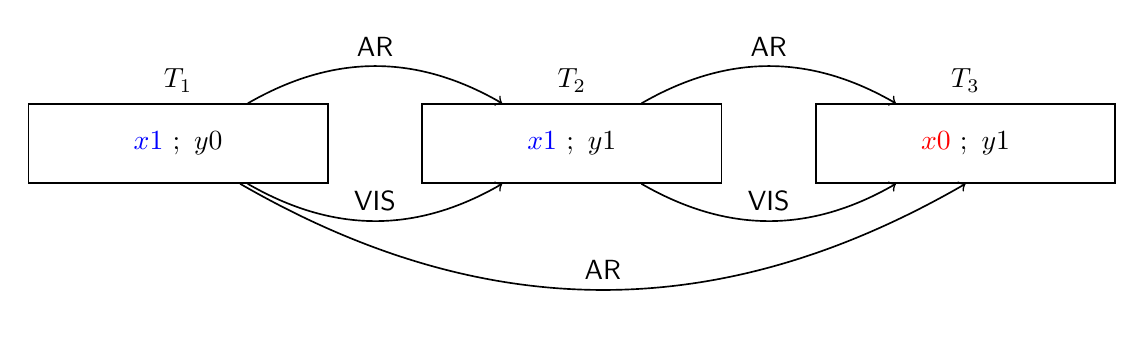
\begin{tikzpicture}[->, semithick]
		\tikzset{
		    trans/.style= {rectangle, draw=black, color=black, minimum width=3.8cm, minimum height=1cm},
		    vis/.style= {above, black!5!black, semithick},
		}
		
		\node[trans] (s1) at (0, 0) {$\textcolor{blue}{\tmwrite{x}{1}}\ ;\ \tmwrite{y}{0}$};
		\node[trans] (s2) at (5, 0) {$\textcolor{blue}{\tmreade{x}{1}}\ ;\ \tmwrite{y}{1}$};
		\node[trans] (s3) at (10, 0) {$\textcolor{red}{\tmreade{x}{0}}\ ;\ \tmreade{y}{1}$};
		\node at (0, 0.8) {$T_1$};
		\node at (5, 0.8) {$T_2$};
		\node at (10, 0.8) {$T_3$};
		
		\draw
		(s1) edge[vis, bend right] node[midway, above] {$\mathsf{VIS}$} (s2)
		(s1) edge[vis, bend left] node[midway, above] {$\mathsf{AR}$} (s2)
		(s1) edge[vis, bend right] node[midway, above] {$\mathsf{AR}$} (s3.270)
		(s2) edge[vis, bend right] node[midway, above] {$\mathsf{VIS}$} (s3)
		(s2) edge[vis, bend left] node[midway, above] {$\mathsf{AR}$} (s3);
	\end{tikzpicture}
	\captionof{figure}{An example of the causality violation anomaly.}
	\label{fig:causVio}
\end{center}
